
\documentclass[10pt,journal,compsoc]{IEEEtran}
\usepackage{graphicx}
\usepackage{epsfig}
\usepackage{multirow}
\usepackage{booktabs}
\usepackage{amsmath}

%\usepackage{xcolor,colortbl}
\usepackage[ruled]{algorithm2e}
\usepackage{amsmath}
\renewcommand{\algorithmcfname}{ALGORITHM}

% *** CITATION PACKAGES ***
%
\ifCLASSOPTIONcompsoc
  % IEEE Computer Society needs nocompress option
  % requires cite.sty v4.0 or later (November 2003)
  \usepackage[nocompress]{cite}
\else
  % normal IEEE
  \usepackage{cite}
\fi

  \usepackage{xcolor,colortbl}
  \usepackage{graphicx}
  % declare the path(s) where your graphic files are
  \graphicspath{{picture/}}

\hyphenation{op-tical net-works semi-conduc-tor}


\begin{document}

\title{Smart Interface: A Hardware Optimizer for Accelerating Heterogeneous Programming}


\author{Chia-Chen~Hsu,
        Chi-Ming~Lee,
        Chih-Wei~Liu,
        Jenq-Kuen~Lee,
        Yarsun~Hsu  % stops a space
\IEEEcompsocitemizethanks{\IEEEcompsocthanksitem C.C. Hsu and J.K. Lee are with the Department of Computer Science, National Tsing Hua University, Taiwan.
\IEEEcompsocthanksitem C.M. Lee and Y. Hsu are with the Department of Electrical Engineering, National Tsing Hua University, Taiwan.
\IEEEcompsocthanksitem C.W. Liu is with the Department of Electronics Engineering, National Chiao Tung University, Taiwan.}% <-this % stops an unwanted space
}


\IEEEtitleabstractindextext{%
\begin{abstract}
Heterogeneous multi-core systems that contain multiple CPUs and GPUs are gaining momentum, as they are providing different computation
power to meet the performance demand of modern applications. On such systems, developers try to fully utilize the computation power both for CPU and
GPU by using the emerging programming models such as CUDA and OpenCL. To achieve the maximal performance, developers must carefully
offload the appropriate workload
to the compute devices according to the characteristics of target architecture.
Under such scenario, seamlessly data motion between different processors become
crucial. Additionally, re-organizing the data layout to fit the target architectures,
such as array-of-structure (AOS) for CPU, structure-of-array (SOA) for GPU,
coordinate (COO) format to ELLPACK (ELL) for sparse computation, diagonal conversion for GPUs, and non-unit stride extraction, address such concern.
%One common issue is coalescing memory accessed for GPU, while array-of-structure (AOS) for CPU versus structure-of-array (SOA) for GPU.
%Another important issue is sparse storage.
%Though coordinate(COO) format is the most general representing storage pattern, it leads to irregular access patterns for GPUs.
%Above cases show that data layout conversion is crucial in heterogeneous systems. However, previous researches present
%software solutions which would not efficiently diminish transform overhead.
%Seamlessly sharing data between processors allows the right processor to handle its appropriate workload and further improves the performance for modern program.
%In this way, seamlessly data motion in heterogeneous system becomes an crucial processing. In many-core GPGPU architectures,
%appropriate data layout of each processor is different causing by individual characteristic.
%As a result, programmers have to reshape data layout frequently to fit different architecture.
In this paper, we propose a hardware memory manager, which efficiently optimizes the conversion of data layouts
for heterogeneous multi-core systems on-the-fly. We address coalescing and sparse format conversion issue in our design.
A novel ping-pong transpose architecture is devised to reorganize non-coalescing access pattern, and a histogram unit and
sparse address generator are presented to process sparse storage format transformation.
Our design reduces the overhead of data transfer and layout transformation among CPU and GPU.
%For general CPU-GPU systems, the smart controller can improve 10x
%performance with negligible area overhead.
%Compared with software-based solution, our design is 2.27$ \times $ faster  in average for adopting benchmarks.
%Testing the scalability of the our design,
%the manager improves 2.42$ \times $ to 45.63$  \times $ from largest data to smallest data.
In our experiment, our design achieves  68.5 to 2.19 speed up comparing to software-based library depending on data size.
%For regular data magnitude, it achieve 16.33 speed up.
Also from the perspective of energy saving, comparing to the software-based solution that uses the whole GPU for data
transformation, our design incurs negligible energy consumption
for both data transfer and transformation.
%Besides, data motion and reordering through the low-cost manager rather than software-based solution , most of the energy is eliminated because of
%the hardware resource gap between the manager and GPU.
%Our design can eliminate most of the energy consumption during data transform and transfer.

\end{abstract}

% Note that keywords are not normally used for peerreview papers.
\begin{IEEEkeywords}
GPGPU, Data Layout Conversion, Heterogeneous System, Memory Locality
\end{IEEEkeywords}}


% make the title area
\maketitle


% To allow for easy dual compilation without having to reenter the
% abstract/keywords data, the \IEEEtitleabstractindextext text will
% not be used in maketitle, but will appear (i.e., to be "transported")
% here as \IEEEdisplaynontitleabstractindextext when the compsoc
% or transmag modes are not selected <OR> if conference mode is selected
% - because all conference papers position the abstract like regular
% papers do.
\IEEEdisplaynontitleabstractindextext
% \IEEEdisplaynontitleabstractindextext has no effect when using
% compsoc or transmag under a non-conference mode.



% For peer review papers, you can put extra information on the cover
% page as needed:
% \ifCLASSOPTIONpeerreview
% \begin{center} \bfseries EDICS Category: 3-BBND \end{center}
% \fi
%
% For peerreview papers, this IEEEtran command inserts a page break and
% creates the second title. It will be ignored for other modes.
\IEEEpeerreviewmaketitle


\IEEEraisesectionheading{\section{Introduction}\label{sec:introduction}}

\IEEEPARstart{R}{eal-time} embedded computing demands both high performance and power efficiency,
as Quality of Service (QoS) and sustainability become its main considerations.
To meet such demands, heterogeneous multi-core systems that utilize more than one
type of processor are recently regarded as effective solutions.
Among them, GPGPU (General-Purpose GPU), which uses massive processing cores in GPU
to handle data-intensive tasks and conventional CPU to perform the sequential ones, is gaining momentum.
Accordingly, OpenCL and CUDA have emerged as programming models that help developers to
dispatch a computational task (kernel) to particular devices in heterogeneous systems.

Today, GPGPU application developers partition programs into multiple
kernels and optimize each of them on target devices with manual efforts.
Take the example of Haar face detection\cite{HAAR}.
It is divided to 22 cascade stages and each stage favors different parallel mechanisms either on CPU or GPU.
Moreover, machine learning is applied to allowing the right processor to handle its appropriate workload by
seamlessly sharing data between cores \cite{partition}. Data would no more stay only in a single processor
but frequently transferring among cores.


However, data motion in heterogeneous systems is not intuitive because
SIMD architectures in GPU implies completely different memory access footprints from those in CPU.
AOS (Array-of-Structure) is typical organization for data
in CPU cores. Consequently, when transplanting purely AOS layout into GPU,
it leads to discontinuous data access pattern and invalidates memory prefetching mechanism in SIMD, hence AOS is considered as non-coalescing layout for GPU.
\cite{CuMAPz}\cite{MemoryThreadLevelParallelism}.
Since such non-coalescing access not only degrades utilization of memory bandwidth, but also collapses system performance, efforts are frequently put into converting non-coalescing layout to coalescing one.


We analyze popular applications and benchmarks \cite{rodinia:} in GPGPU and categorize
non-coalescing access issues in heterogenous systems as below:

\begin{itemize}
  \item \textbf{AOS, SOA and ASTA} The organization of structure and array affects memory throughput significantly. Figure \ref{fig:ap_benchmark}.(a) gives the motivating example for the performance
difference in GPU via AOS, SOA(Structure-of-Array) shape \cite{MemoryAccessPattern}, and
ASTA(Array-of-Structure-of-Tiled Array) \cite{ASTA}.
As shown in Figure \ref{fig:ap_benchmark}(a), SOA and ASTA version of data layout create 3-13 performance speed up over AOS on NVIDIA GT460 by CUDA 4.2.
Comparing to the AOS layout used in CPU, the layout reshape is needed for GPU processing.
  \item \textbf{Sparse matrix} Non-zero elements of sparse matrix can be efficiently computed and further improves overall performance by
reshaping storage format. Nevertheless, the most general representing sparse format is coordinate (COO), while
the general agreed suit storage format in GPU is ELLPACK (ELL) \cite{AdELL}\cite{AutoSpMV}.
Figure \ref{fig:ap_benchmark}(b) evaluates the SpMV kernel applications with COO format compared to ELL format.
SpMV with storing ELL format matrix achieves 4.77 to 1.22 speed up than COO format, and similar result is also reported in the literature \cite{spmv_CUDA}.
  \item \textbf{Dynamic programming} Dynamic programming (DP) is a popular technique to solve optimization problems. To perform DP in GPU,
developers firstly model the problem by constructing a matrix. Then, GPU threads fill out the matrix
by traversing from left-top to right-bottom diagonally. Since the memory footprints of GPU threads are
diagonal strides rather than regular one, such data layout leads to non-coalescing access likewise.
  \item \textbf{Non-unit stride} In many GPGPU applications, we often transfer chunk of data but only fraction of them are accessed by GPU. Since these useful data are spaced with certain intervals that hold useless ones, the memory footprints of GPU threads are non-unit strides. Such data layouts can also be considered as non-coalescing ones because any useful data is always followed by useless one.
\end{itemize}



%This result shows the benefit of layout transformation from COO to ELL.
%related work on coalecsing issue



To solve the non-coalescing access problem,
research efforts include off-line compiler frameworks to transform GPU programs
to be with  right access patterns \cite{AffineLoop}.
According to Amdahl's law,
the data motion and layout reshape in different processing units are considered
overhead and should be minimized whenever possible.
In this regard, the effort includes the work
to eliminate non-coalesced accessing memory pattern by data reorganization.
%Data layout transformation would improve the localizing memory access in nonuniform memory architecture\cite{ASTA_old}.
The work in \cite{ModelDrivenSpMV}\cite{AutoSpMV}
proposes appropriate data layout and optimal kernel parallelism for sparse matrix applications.
Sung \textit{et al.} \cite{ASTA} proposed a novel data layout, ASTA,
and an in-place marshaling algorithm for
 improving the memory access for GPU applications.
Che \textit{et al.} \cite{Dymaxion} proposed Dymaxion API to
optimize memory access patterns and hide the overhead through chunking
and overlapping with PCIe transfer.
%With the software solvers,
%the transpose overhead still inevitably exists in these systems.
% % % % % % %sparse matrix
%Another issue we address is sparse matrix storage format in GPUs.
Monakov \textit{et al.} \cite{AutoSpMV} modified present ELL format and propose a new sliced-ELL format for parallel GPU programming.
Maggioni \cite{AdELL} proposed a novel Adaptive ELL format with warp-balancing programming algorithm.
With the software solvers, the transpose overhead still inevitably exists in these systems.
%However, above researches did not
%illustrate the method for converting data layout.
%Cusp\cite{Cusp} is a software library witch supports sparse matrix
%conversion between several formats.
% % % % % % % % % % % %memory controller
We explore the research direction in the hardware solution
in this work to aim at reducing the layout reshape overhead.
Exploiting hardware solvers in multi-processor memory connection is an
advisable choice which provides a prime way to optimize
overall architectures.
For example, in the past, Saidi \textit{et al.} \cite{Cell} proposed an
optimized off-chip memory
to local memory DMA to enhance the communication in multi-cores.
Jeong \textit{et al.} \cite{QoS-Aware} proposed a Quality of Service
memory controller to enhance the hit rate of DRAM when data transferring
between CPU and GPU.

% % % % % % % % % % % % % % % % % % % % % % % % %

To improve the efficiency of data reorganization in heterogeneous systems, we develop a hardware-based memory optimizer,which processes data motion appending data reorganization.
To the best of our knowledge, this is the first hardware demonstration
for data layout conversion.
With the master IP, SC (Smart Controller), connecting with CPU-GPU systems,
our design reshapes data layout such as AOS, SOA, and ASTA
during data move between the host and device.
The proposed transpose circuit shuffles data block-by-block. By ping-pong transpose units operating
synchronous-pipeline and the address generator performing
formulaic out-of-order address mapping scheduling, the proposed SC manager
achieves layout transpose with efficiency.
The proposed memory manager can also transfer and convert a subset of source data instead of the full set of data, which benefits some applications that just need a subset of the original data. It also supports diagonal conversion, which can help applications, such as dynamic programming, that needs to turn data plane into 45 degree.

Besides, we propose a 2-step sparse matrix layout converter to automatically reshape sparse format from COO to ELL.


Moreover, we support an API for programmers to bi-directionally
%Moreover, our design allows bi-directionally
transfer and transpose data between CPU and GPU.
In our experiment, the memory manager is implemented
by UMC 65nm CMOS technology. To evaluate the performance of SC,
post-synthesis level simulation is adopted with simulated host
and device memory model. PTTWAC library \cite{ASTA} is adopted
on NVIDIA GT460 GPU for performance comparison.
SC transposing attached with transfer operation performs approximately
68.5 to 2.19 times speed up depending on data size
over the best available software solution in \cite{ASTA}.
The memory manager also shows 2.6 to 1.7 times speed up than \cite{Dymaxion} when converting data to diagonal patterns, and shows XX times speed up than performing in GPU when stride conversion.
On the side of sparse format conversion, SC performs
2.42 times in average over other software-based library \cite{Cusp}.
Moreover, our design
provides a significant power reduction compared to software-based
solution that uses the whole GPU for data transformation.


%we implement a smart memory controller(SC), which transposing data layout on the way that data move from CPU to GPU.

The rest of this paper is organized as follows:
%In Section \ref{cha:background}, we introduce the origins of coalescing access in GPU and %introduces the ASTA layout.
Section \ref{cha:architecture} reveals architecture of SC. Section \ref{cha:Advanced} further illustrates the
advanced design issues of SC. Section \ref{Special patterns} shows the special patterns that SC supports, including stride, diagonal, and sparse.
%Section \ref{cha:TTI} proposes an extend
%CUDA API for applying SC to reshape data layout on-the-fly.
%\iffalse Section \ref{kernel rewriting} illustrates the kernel application rewriting to obtain  better performance collocating with coalesced data shape.\fi
%Related works is discussed in section\ref{related work}.
Design synthesis and experiment results are revealed in Section \ref{cha:experiment}. Finally, Section 6 concludes the contribution of this paper.


\begin{figure*}[htb]
\footnotesize
\begin{center}
\graphicspath{{picture/}}
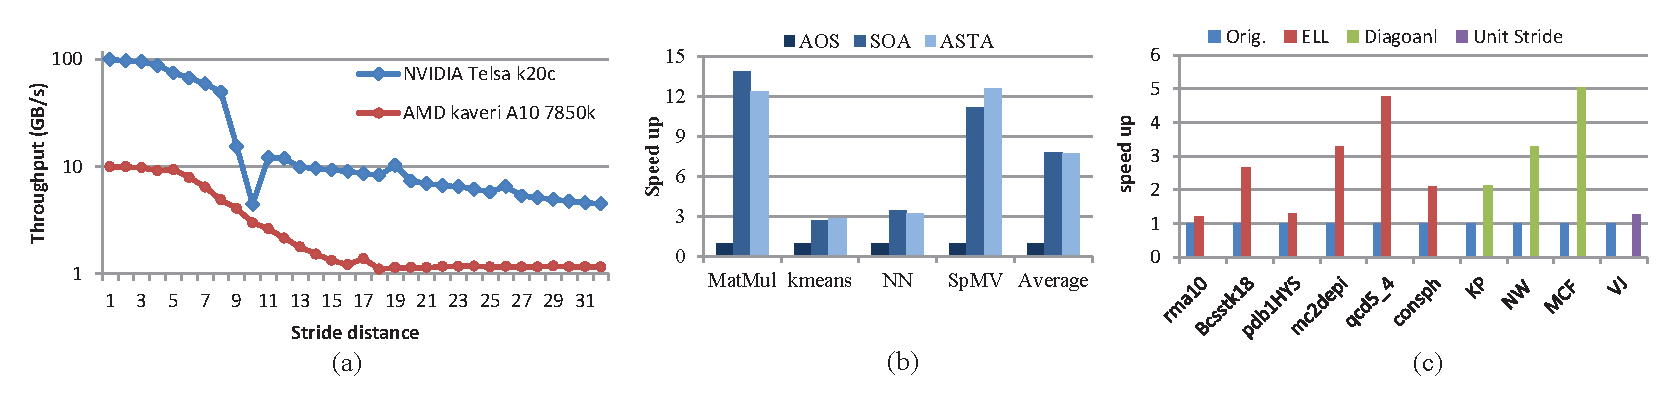
\includegraphics[scale=0.6]{motivation_benchmark}
\caption{Kernel application execution speed up in GPU (a) performance comparison among AOS, SOA and ASTA type of data layout (b) performance comparison among COO and ELL storage format for SpMV applications}
\label{fig:ap_benchmark}
\end{center}
\end{figure*}

\section{Architecture of Memory Manager}\label{cha:architecture}
To deal with data conversion issues, previous works utilize software library to reshape data structures.
Data layout is transposed before or after data transfer, either performed by CPU or GPU. In this section,
we present our proposed  smart controller (SC) with ping-pong transpose unit as the optimized memory access manager.
The manager performs data reorganization during data transfer, which can almost eliminate all the reorganization overhead.

\subsection{System Overview}
%Figure \ref{fig:system} (a) is the integration prototype of our design, SC is connected to system bus as a master IP.
%In current heterogeneous systems, GPU operation is a slave (device) which is attached to a master (host) CPU processor.
%Before GPU operates, CPU requires to send data to GPU from bus. In our approach, SC would play a intermediary bridge for
%data transfer and automatically reorganize data layout between host and devices. When SC request is triggered by API, CPU (host)
%and main memory would send data and API parameters to SC, then send to GPU in pipeline manner. After SC processed, optimized data layout is stored in global memory of GPU.
%Then optimized layout would improve GPU kernel performance.
The integration of such a SoC system needs a wrapper to be the connection between IP and
systems, and it could reference \cite{ROSES_DAC}\cite{ROSES}.

The architecture of our proposed manager is illustrated in Figure \ref{fig:system}. Such a design could be connected
to the system bus as a master IP with some wrappers \cite{ROSES_DAC}\cite{ROSES}.
We have two main types of layout converter, address coalescing and sparse matrix.
For the part of coalescing converter, we have transpose units (TU) with source/destination address generator (AG).
TUs are designed for fixed-size transpose. A pair of TUs are bounded in a ping-pong manner to reduce latency.
AGs are required to generate memory access patterns to host and device. The sparse converter contains
a histogram unit and a sparse format generator for format conversion.
All the transpose units and address generators are controlled by a centralized control unit. A smart controller library API is provided, which allows programmers to specify memory copy
with or without transpose operations using the proposed controller in high-level programs.
The syntax of memory copy operations in the smart controller library is resemble to conventional memory copy operations except for additional options for transpose and non-blocking mode.

\begin{figure}[t]
\begin{center}
\graphicspath{{picture/}}

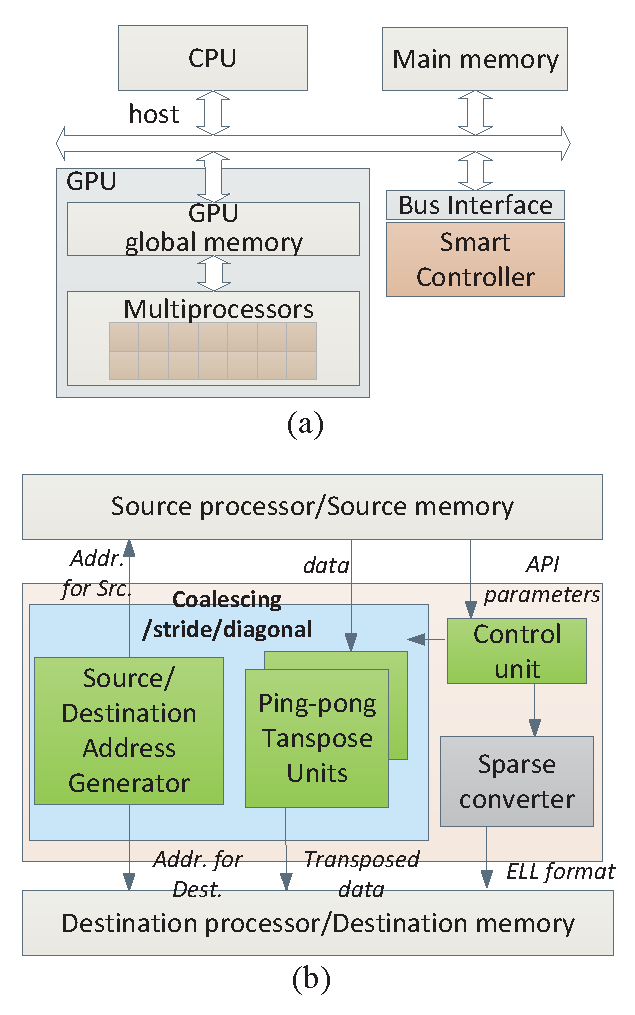
\includegraphics[scale=0.6]{SystemOverview_architecture_v03}

\caption{System overview (a)SC integration with system (b)block diagram of SC}
\label{fig:system}
\end{center}
\end{figure}

The execution flow of SC is illustrated in Algorithm \ref{alg:SC}.
Once a memory copy request with transpose from source processor ($ P_{s} $) is fired, the control unit distinguishes the $ mode $ signal.
In $ Transpose $ or $ Reversion $ mode,
the control unit schedules memory access and transpose operations to perform transposing on scalable data sets in a pipelined manner.
For data importing, source AG generates the address and sends the request to $ P_{s} $, and in the next cycle the burst data imports to TU,
as  described in line 6-11. For data exporting, TU outputs data and destination AG generates the address simultaneously, as shown in line 12-16.
Importing and exporting data are executed with synchronized-pipeline by ping-pong transpose units. A more detailed design of synchronized-pipeline transpose units will be illustrated in Section \ref{cha:PPTU} shortly.

In $stride$ and $diagonal$ mode, the mechanisms are similar to  $ Transpose $ or $ Reversion $ mode but the controller use modified TU and AG, we will discuss then in detail in Section \ref{Stride} and Section \ref{Diagonal}.
In $ SparseConvert $ mode, the sparse format converter is triggered.
The Histogram Unit is designed to calculate maximal non-zero elements per row sequentially. ELL format generator generates
ELL format address space while data input with COO order, and this function is invoked twice for generating both column array and value array. The detailed architecture of sparse converter is showed in Section \ref{sparse}



\begin{algorithm}  [h]
%\linesnumbered
%\scriptsize
%\footnotesize
\KwIn{
Parameters from memcpySC() API:
 mode is the layout transpose type, non-blocking signal, and parameters depending on conversion type}
%Source-layout plane,$S(i,j)$, where i=0,1,2,..., $S_{a} $, and j=0,1,2,..., $S_{s}$.}
\KwResult{
%Transformed destination layout plane, $ D(i',j') $, where $ i' $=0,1,2,..., $S_{tile} $, and $ j' $=0,1,2,..., $S_{s}\times tile\_num$.}
Transformed data layout stored in the destination memory}


\Begin{
  request from source processor($ P_{s} $);  \\
	\Switch{mode}{
			\uCase{Coalescing , Reversion}{
				 \ForPar{ !the last data }{
					 \For	{$i\leftarrow 1$  \KwTo  $S_{m}$}{
					 	AddressGenerator(mode, source);\\
					 	\If{ping\_in}{
					 			 		Import burst data to Ping-TU();}
					 	\ElseIf{pong\_in}{
					 			  		 Import burst to  Pong-TU();}		 		
					 }
				 }
				\ForPar{$j\leftarrow 1$ \KwTo $S_{n}$}{
						AddressGenerator(mode, destination);\\
					\If{ping\_in}{
							   		Export burst data from Ping-TU();}	
					\ElseIf{pong\_in}{
							    		 Export burst from  Pong-TU();}		   		
				}
			
            \uCase{Advanced Patterns}{
			    Advanced patterns():\\
			}				
		
			}		
	}
	 send  the non-blocking signal back to $ P_{s} $ ; 	
 }



%\caption{SmartController ($ S_{s},  S_{a}, S_{tile}, mode $ )}
\caption{ Smart Controller(SC) }
\label{alg:SC}
\end{algorithm}




\subsection{Control Unit}
With a goal to achieve a high flexible and scalable design, the design of the control unit (CU) is important. In this subsection, we introduce the control mechanisms of our design. After SC is triggered, CU would generate corresponding control signals to conduct SC according to the input parameters.
We describe each parameter below.




\begin{itemize}

\item \textbf{Size }
We define a descriptor $ (S_{a}, S_{s}) $, which presents the under-transposed layout with structure size, $ S_{s} $, and array size, $ S_{a} $. Structure size, $ S_{s} $, is also the stride distance of original AOS layout. Array size, $ S_{a} $, is the number of structures.
To transpose source data layout  $(S_{a}, S_{s}) $ by TU $(S_{n}, S_{m})$, let $ l_{s} $ represent $ |\frac{S_{s}}{S_{m}}| $ and let $ l_{a} $ represent $ |\frac{S_{a}}{S_{n}}| $.
if $ l_{a} < \bigcap l_{s}<1 $, the control unit assigns a single transpose unit for transposing instead of Ping-Pong pairs TU to reduce power consuming. Instead, if $ l_{a}>1 \bigcup l_{s}>1 $, CU exploits a pair of transpose units performing ping-pong like operations to accelerate the transformation process.
% The above description is used for TU-based conversion: Coalescing, Stride, and Diagonal. For Sparse converter, the size is
\iffalse
Apart from burst capacity in data access and retreat, the transpose unit also realize out-of-order specify to minimize the stall time between in and out. This mechanism controlled by control unit.
\fi
\item  \textbf{Transpose Mode}
Proposed SC provides not only transposing functions between AOS and ASTA/ SOA but also directly transferring usages with normal mode. We define the data reorganization from source layout to object layout as $ source \rightarrow object $. The supported mode is shown in Table ~\ref{fig:API}%~\ref{tb:ControlParameter}.
If a $ normal $ mode is chosen, Ping-Pong TU would not be triggered. In other words, data would be sent from host to device straightly without passing PPTU. By this clock-gating mechanism, the system could have the advantage of power saving. If $ transpose $ or $ reversion $ mode is chosen, CU conducts AG to generate suitable source/destination addresses. Apart from regular layout conversion, we also support irregular layout conversion. If $DiagonalConvert $ and $Stride$ mode is triggered, CU exploit enhanced the Transpose Unit and Address Generator to handle layout reorganization. If $SparseConvert $ mode is chosen, CU conduct sparse storage format generator to calculating ELL address space.

\item  \textbf{Direction}
Data transferring between host and device is a mutual communication. Let the descriptor of transferring direction be $ source\rightharpoonup destination $. We support two kinds of directions. Control unit is in charge of connecting source-destination pairs to homologous system memory. By this mechanism, SC achieves multi-directional transmitting.

\end{itemize}



\subsection{Transpose Unit}
\label{cha:TU}


Transpose-appended data motion is processed block-by-block, and the transpose unit (TU) is designed to transpose a specific size of block.
To decide an appropriate size for TU, available memory bandwidth of CPU and GPU needs to be taken into careful consideration.
The best utilization for bandwidth is to keep the data flow in a burst.

Suppose that the available CPU memory bandwidth is \textit{c} bytes, GPU global memory bandwidth is \textit{g} bytes, and data width is \textit{w} bytes, we define transpose unit is the size of $ (S_{n}, S_{m}) $, where $ S_{n}=c/w $ and $ S_{m}=g/w $.


This setting promises the import and export of TU are adapted to the memory bandwidth without any wasting.
The architecture of TU is shown in Figure \ref{fig:TU} and the execution behavior is illustrated in Algorithm \ref{alg:TU}. It is primarily composed of $ S_{m}$ banked memory that each bank can hold $ S_{n} \times w $ bytes with  input burst. When data inputs from memory, $  sel\_in $ signal chooses one bank to allocate data, as shown in line 2-4. After $ S_{m}$ cycles, $ S_{m}$ banks are filled, and TU turns to operate output, as seen in line 5-7. When data exports from TU, TU relies on the $ sel\_out $ signal to choose one w-byte-vector from each bank and generates an $  S_{m}\times w $ byte output.

\begin{figure}[tb]
\begin{center}
\graphicspath{{picture/}}
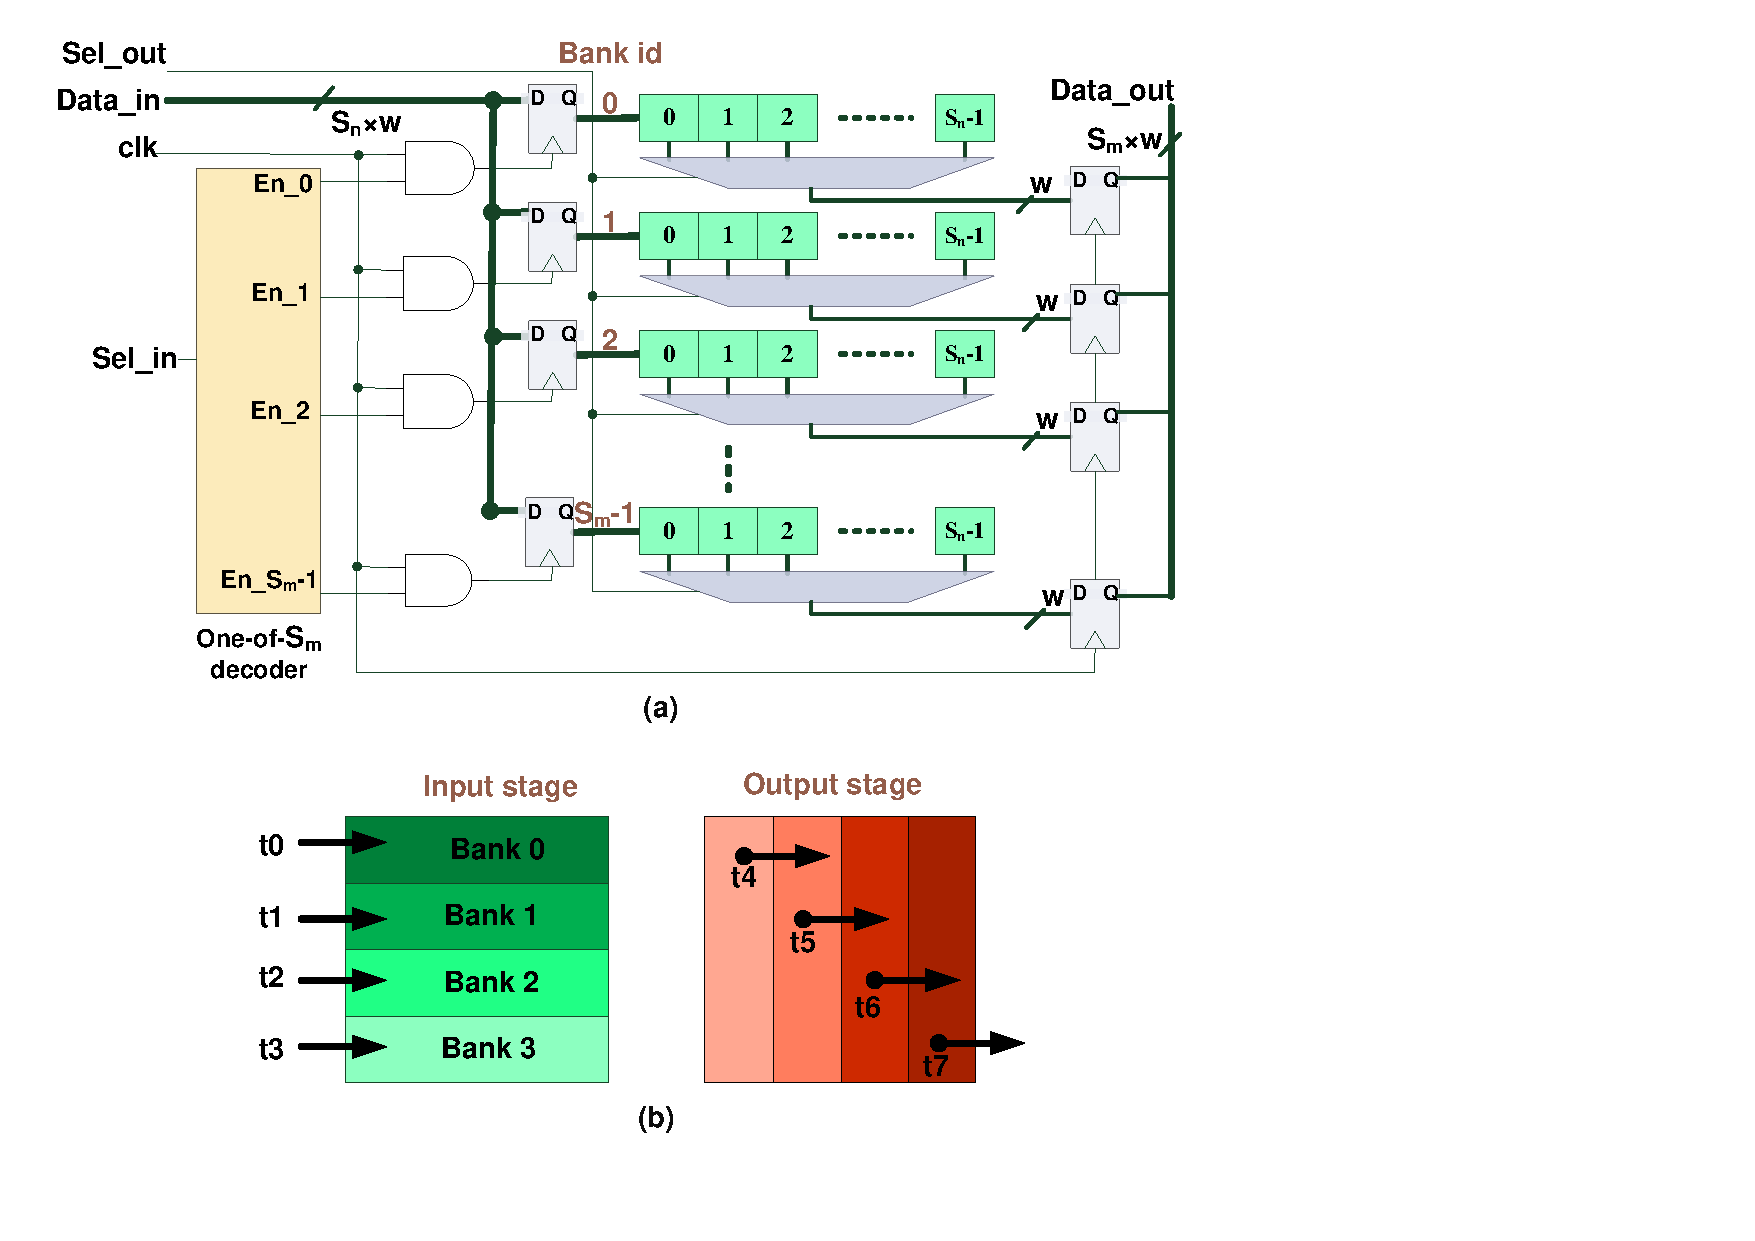
\includegraphics[scale=0.4]{TU_v02}
\caption{Architecture of transpose unit}
\label{fig:TU}
\end{center}
\end{figure}

\begin{algorithm} [h]
%\linesnumbered
%\scriptsize
%\footnotesize
\KwIn{
%$burst\_in $ is a continuous data accessed from source memory}
Block of origin data from source memory}
\KwResult{
%$burst\_out $ is a continuous data that would be sent to destination memory}
Block of transformed data to destination memory}
\Begin{
\If{Out\_done}{
   \For{$i\leftarrow 1$ \KwTo $S_{m}$}{
	  Fill $ S_{n}\times w $ byte burst data into bank i;\\
	  }
  }
 \If{In\_done}{
  \For{$j\leftarrow 1$ \KwTo $S_{n}$}{
  	  Choose $ j_{st} $ data from each bank to generate $ S_{m}\times w $ byte burst data.
    }
    }
}
\caption{Transpose Unit()}
\label{alg:TU}
\end{algorithm}

%===================Control Unit===================


%===================Sparse Converter===================

%===================Interface===================
\subsection{Software Interface}
%As we mentioned earlier,

To wake up the manager, a convenient way for programmers is to apply a software API.
We integrate our hardware converter in systems by a API connection mechanism, performing bi-directionally transfer and transpose data between CPU and GPU.
%to bi-directionally transfer and transpose data between CPU and GPU.
The programmer could exploit the proposed API to wake up the memory access manager for data
reshaping. The proposed APIs are shown in Table \ref{fig:API}. It is extended from
CUDA API, $ cudaMemcpy()$.
We added several parameters, which are $ mode $,  \textit{nonblocking-signal}  , and $parameters$.
The $mode$ parameter indicates the behaviors of SC, which could be \textit{Normal}, \textit{Transpose}, \textit{Reversion}, \textit{SparseConvert},  \textit{DiagonalConvert}, and  \textit{Stride}.
The \textit{nonblocking-signal} parameter is used to inform the source device for the accomplishment of data motion.

$parameters$ are required information depending on $ mode $.
For \textit{Transpose}, \textit{Reversion} mode, which are
 primarily for coalescing transformation (AOS, SOA and ASTA),  $ Array\_size $,
 $ Structure\_size $, and $ Tile\_size $ are required parameters.
$Array\_size$ and $Structure\_size$ are data size and
$Tile\_size$ represents the target tile size of ASTA structure.
 For \textit{SparseConvert} mode, $ Numbers\ of\ row $, $ column $ and   \textit{Numbers of non-zero elements}  are parameters to generate  ELL format.
 For  \textit{DiagonalConvert} mode, programmers use parameters to define the direction of rotation is clockwise or counterclockwise.
 For \textit{Stride} mode, the parameter is the step length.

\begin{table}[]
\renewcommand{\arraystretch}{1.3}
\centering
\caption{Application Programming Interface of Smart Controller }
\label{fig:API}
\begin{tabular}{|l|l|}
\hline
\multicolumn{2}{|l|}{\begin{tabular}[c]{@{}l@{}}memcpySC(void *dst, const void *src, size\_t count, MemcpyKind,\\ \textbf{mode, nonblocking-signal,parameters})\end{tabular}}             \\ \hline
\hline
\multirow{6}{*}{mode}                                         & Normal: transfer data without transpose                                                                          \\ \cline{2-2}
                                                              & Transpose: perform AOS $\rightarrow$ ASTA /SOA                                                                                 \\ \cline{2-2}
                                                              & Reversion : perform ASTA /SOA $\rightarrow$ AOS                                                                                \\ \cline{2-2}
                                                              & SparseConvert: perform COO $\rightarrow$ $ ELL_{SOA} $\\ \cline{2-2}
                                                              & Diagonal: turn data plane to 45 degrees                                                                   \\ \cline{2-2}
                                                              & Stride : gather together data with non-unit stride                                                               \\ \hline
\begin{tabular}[c]{@{}l@{}}nonblocking\\ -signal\end{tabular} & Check signal to ensure data security                                                                             \\ \hline
\end{tabular}
\end{table}

%====================================================

%===================================================
\section{Detailed Design Considerations}
\label{cha:Advanced}
The architecture of the hardware design determines the system performance indeed. In this section, some optimizations are revealed for improving hardware performance.

\subsection{The Design of Transpose Unit}

The intuitive way to rearrange data between two memory models is using address remapping directly without any register.
However, this kind of scheme would not fully utilize memory bandwidth because of separate address mapping.
The best utilization for bandwidth is to keep data flow in a burst, as described earlier in Section  \ref{cha:TU}.
In our design,  we define transpose unit size as  $  (S_{t}, S_{t}) $, where $S_{t} =min(S_{n},S_{m})$, instead of $  (S_{n}, S_{m}) $ for two reasons.
First, although TU $ (S_{n}, S_{m}) $ promises the import and export of transpose unit are adapted to the memory bandwidth without any wasting, TU $  (S_{t}, S_{t}) $ could perform similar throughput with negligible latency but lower area.
Second, by adopting the same size in/out ports,
TU achieves bidirectional data motion.
In our experiment, while the configuration of system bandwidth is 64 bits and DRAM bandwidth of GPU is 256 bits.
%Take our experiment setting as an example, system bandwidth is 64 bits, while  DRAM bandwidth of GPU is 256bits, the performance of these two schemes is shown in the LHS of Figure \ref{fig:SC_design_comparison}.
Our approach only increases negligible latency while it saves up to 75\% of area via adopting  TU $  (S_{t}, S_{t}) $.

\subsection{Synchronous-Pipeline by PPTU}
 \label{cha:PPTU}
While host and device could transmit data by their bus simultaneously, a single TU could only process export or import at one time. Hence, we arrange ping-pong pairs transpose units (PPTU) to perform synchronous-pipeline in and out. The data motion, which PPTU performs, could be seen in Figure \ref{fig:PPTU}. Let the transpose unit size of TU be (4, 4), and we record time period from \textit{t=0} to \textit{t=11}. When \textit{t=0} to \textit{t=3}, Ping TU imports data. During \textit{t=4} to \textit{t=7}, Ping TU turns to export data and Pong TU starts to import data. From \textit{t=8} to \textit{t=11}, Ping TU imports data again and Pong TU exports data. We could also notice that, in Figure \ref{fig:PPTU}, import is in a horizontal way but export is in a vertical way. This manner is coordinated with Figure \ref{fig:TU}. Horizontal input represents import  fits in a bank, and vertical output means exporting a vector from each bank.
%The performance improvement of PPTU could be seen in Figure \ref{fig:SC_design_comparison}. PPTU performs better than the single TU case.
Through the interleaved operation of Ping TU and Pong TU, SC reaches synchronous-pipeline and performs twice as fast than single TU.

 \begin{figure}[htpb]
 \begin{center}
 \graphicspath{{picture/}}
 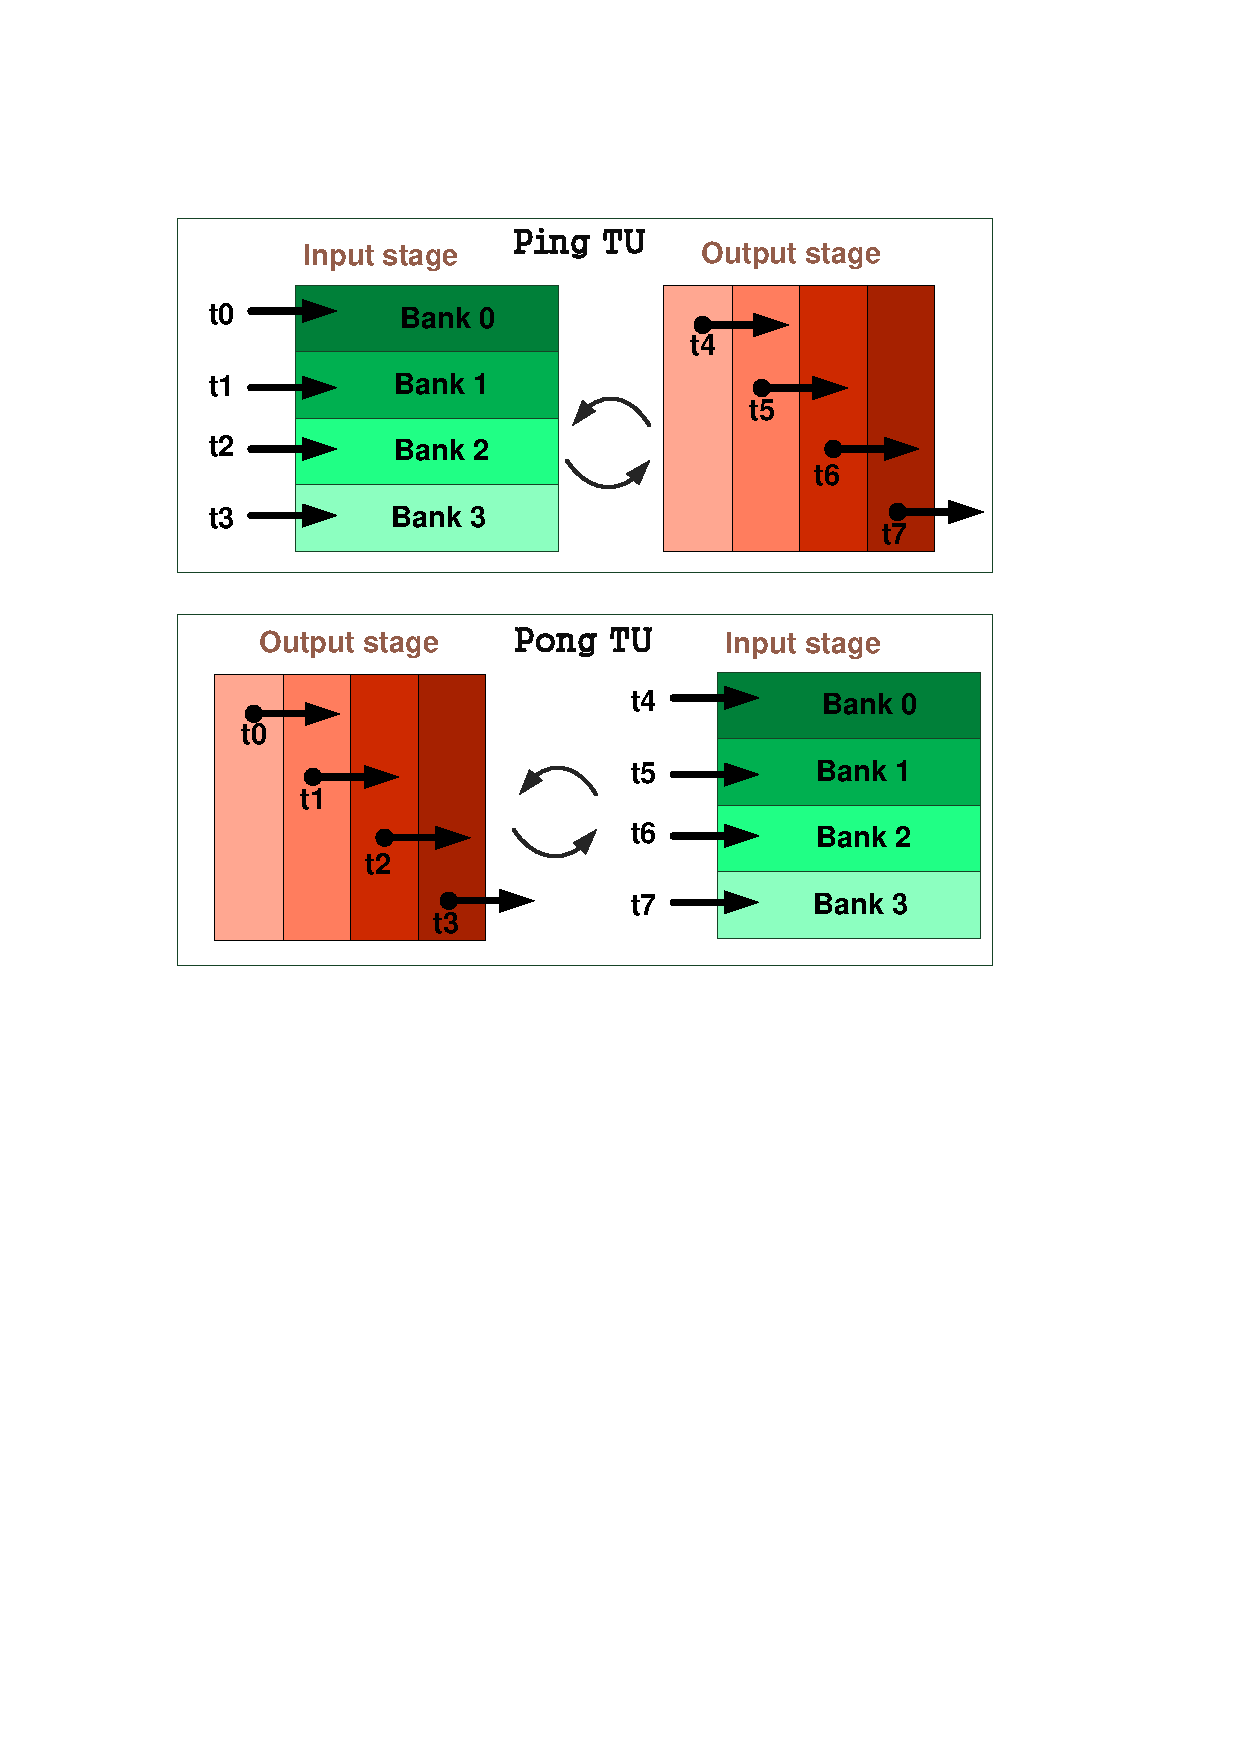
\includegraphics[scale=0.5]{PPTU_v02}
 \caption{Synchronous-pipeline data flow }
 \label{fig:PPTU}
 \end{center}
 \end{figure}

\subsection{Out-of-Order Data Flow}
The rule to access data from source memory and output data is scheduled by AG.
A well-designed AG guarantees the system pipeline without stall.
To achieve this goal, accessing pattern and storing pattern must be taken into considerations mutually.
AG handles out-of-order data flow to achieve data structure reorganization.
The rule of out-of-order data flow is listed in Algorithm \ref{algo:AG}. The mapping address definition of coalesced/non-coalesced data layout is revealed in lines 15-16.
Let source data layout size be $ (S_{a}, S_{s}) $, transpose unit size be $ (S_{t}, S_{t}) $, and tile size be $  Tile  $.  We have $ tile\_num = S_{a}/Tile $, which means the number of tiled tile-of-structure. In addition, we have $ l_{tile}=Tile/S_{n} $, which indicates the number that TU would be needed to fit the tiled edge.   We also have $ l_{s}= S_{s}/S_{t} $, which indicate the number the TU would be needed to fit the $  S_{s}  $ edge.
For both source and destination layout plane, AG perform four-phase data scanning : $ w,\ k,\ j,\ i $, as shown in Lines 3-4.
%We design AG with the principle of regular-oriented.
To illustrate the operation of the AG, we take an example which performs a reorganization from non-coalesced AOS layout in source memory to coalesced ASTA layout in destination memory, as shown in Figure \ref{fig:Out-of-Order}.
For the non-coalesced source part of layout, data motion follows the address assignment of $ Idx\_NonCoalesced $ which decided by Line 7.
The first phase, $ w $, presents scanning a block, and a block is fitted the size of TU. Then, moving a block of data in column-major format presents the second phase, $ k $.
After scanning a tile-of-block, jumping to next column is phase $ j $.
It will stay in phase $ j $ until cumulatively scanning a tile-of- structure, and this is phase $ i $.
On the other hand, for the coalesced destination layout, data motion follows the address arrangement of $ Idx\_Coalesced $ which decided by Line 12. Firstly, the $ w $ phase presents storing a block, and  then AG vertically moves each TU block to destination by second phase, $ k $. After moving $S_{t}\times S_{s}$ numbers of data, third phase, $ j $, leads the motion to shift right in $S_{t}$ steps and continuously storing a thin-tall data layout. Finally, when AG finishes storing $Tile\times S_{s}$ data, phase $ i $ performs the next cycle of moving tile-of $S_{s}$ data.
By our mechanism, layout reorganization performs in a regular manner with no stall time.
%We also provide the bidirectional method for address generation.

\begin{figure}[bt]
\begin{center}
\graphicspath{{picture/}}
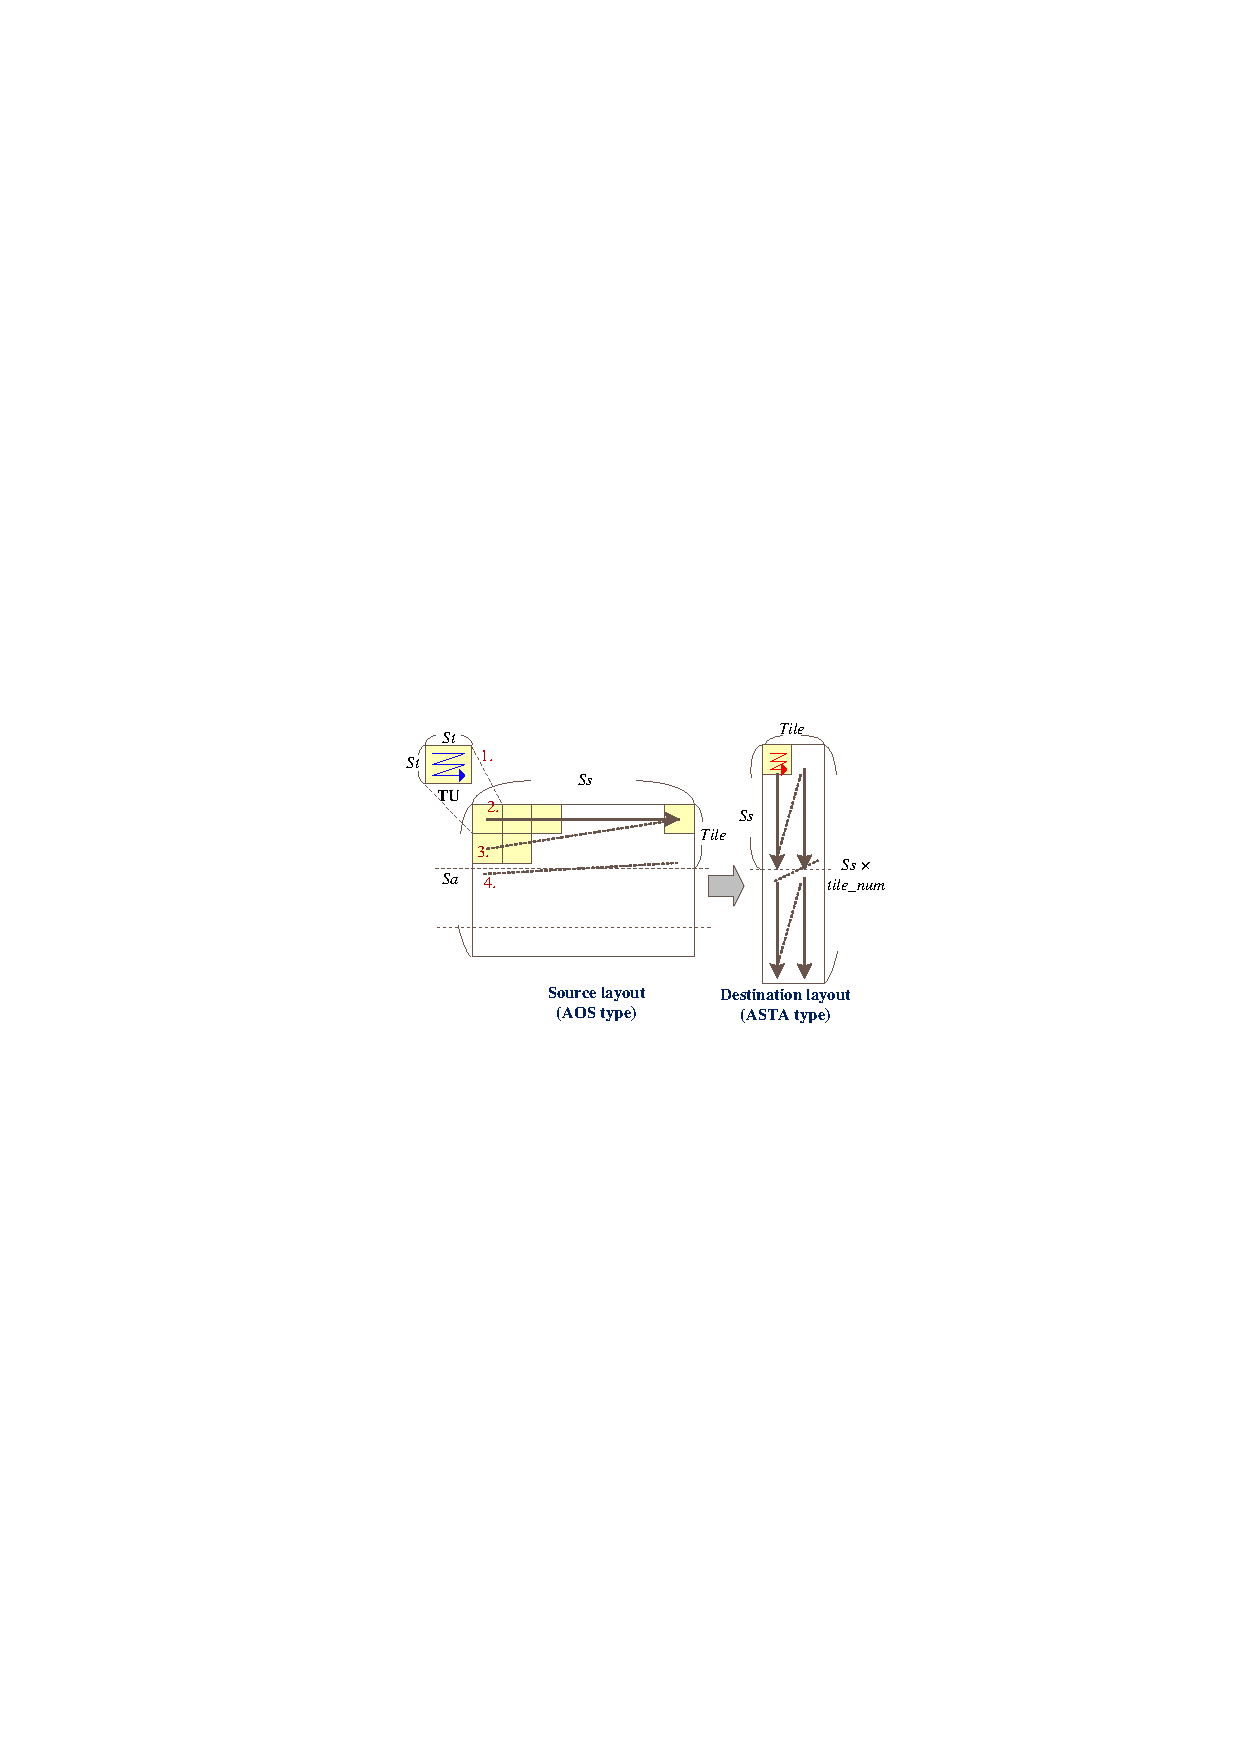
\includegraphics[scale=0.8]{Out_of_Order_v2}
\caption{Out-of-order data motion between source memory and destination memory}
\label{fig:Out-of-Order}
\end{center}
\end{figure}

\begin{algorithm}[tb]
\caption{Address Generator}
%\scriptsize
\footnotesize
\label{algo:AG}
%\end{center}
%\footnotesize
\textbf{Input:} $  mode,l_{tile}, l_{s}, S_{n},tile\_num $

\textbf{Output:} $ addr\_src$, and $addr\_dest $

%\textit{\textbf{In each cycle}}

% \Begin{	
        \ForEach{i=1 to  $tile\_num$,
        		j=1 to $l_{tile}$,\\
        		 k= 1 to $l_{s}$,
        		 w= 1 to  $S_{t}$}{
        		 \If {plane==Source}{
        		 \If {mode==transpose}{
     				 $ addr\_src$=	Idx\_NonCoalesced;
                    }
                    \ElseIf {mode==reversion}{
                  	  $ addr\_src$= Idx\_Coalesced;				
                                  }
                  }
                   \ElseIf {plane==Destination}{
                          		 \If {mode==transpose}{
                       			$addr\_dest $ =	Idx\_Coalesced;
                                      }
                                      \ElseIf {mode==reversion}{
                	$addr\_dest $ = Idx\_NonCoalesced;				
                                                    }
                                    }
         }

 %     }
% Idx\_NonCoalesced $ \leftarrow $ w $\times$$S_{s}$ + k$\times$$S_{t}$+j$\times$$S_{t}$$\times$$ S_{s} $ +i$\times$$ Tile $$\times$$ S_{s} $ \\
% Idx\_Coalesced $ \leftarrow $ w$\times$$ Tile $+k$\times$ $S_{t}$$\times$$ Tile $+j$\times$$S_{t}$ +i$\times$$ Tile $$\times$$ S_{s} $ 	

$Idx\_NonCoalesced  \leftarrow  w \times S_{s}+
k \times S_{t} +j \times S_{t} \times  S_{s}  +i \times  Tile \times S_{s}$

$ Idx\_Coalesced \leftarrow  w \times Tile +k \times S_{t}\times Tile +j \times S_{t}+i \times Tile \times S_{s}$

\end{algorithm}

For better understanding of out-of-order data fetch and data flow in ping-pong transpose units,
 we provide a case study for it. Suppose transpose units ($S_{n}, S_{m}$) = (2, 4), and source data layout ($S_{A}, S_{S}$) = (4, 8), the lifetime analysis for ($S_{A}, S_{S}$) is presented in Figure \ref{fig:Out-of-Order_Example}. Figure \ref{fig:Out-of-Order_Example}, we reveal the data import and export from transpose unit.
 Data in source memory address addr\_src is presented as d\_src(addr\_src), and data in destination memory address addr\_dst is presented as d\_dst(addr\_dst).
  Green and blue grids present transpose unit ping and transpose unit pong respectively. In addition, deep color and light color separately performs import and export and gray area means data is in the transpose units.
 We take the first entire period of Ping TU as a example.
 From cycle 0 to cycle 3, d\_src(0-1), d\_src(4-5), d\_src(8-9), and d\_src(12-13) are transferred into ping TU.
Then, they are reordered and sent to d\_dst(0-3) and d\_dst(8-11) at cycle 4 and cycle 5.
At the same time, the pong TU synchronously receives d\_src(2-3), d\_src(6-7), and these data will be transferred into destination memory after the pong TU is full.

 This experiment clearly present data flow and how ping-pong transpose units handle overall data layout.

\begin{figure}[bt]
\begin{center}
\graphicspath{{picture/}}
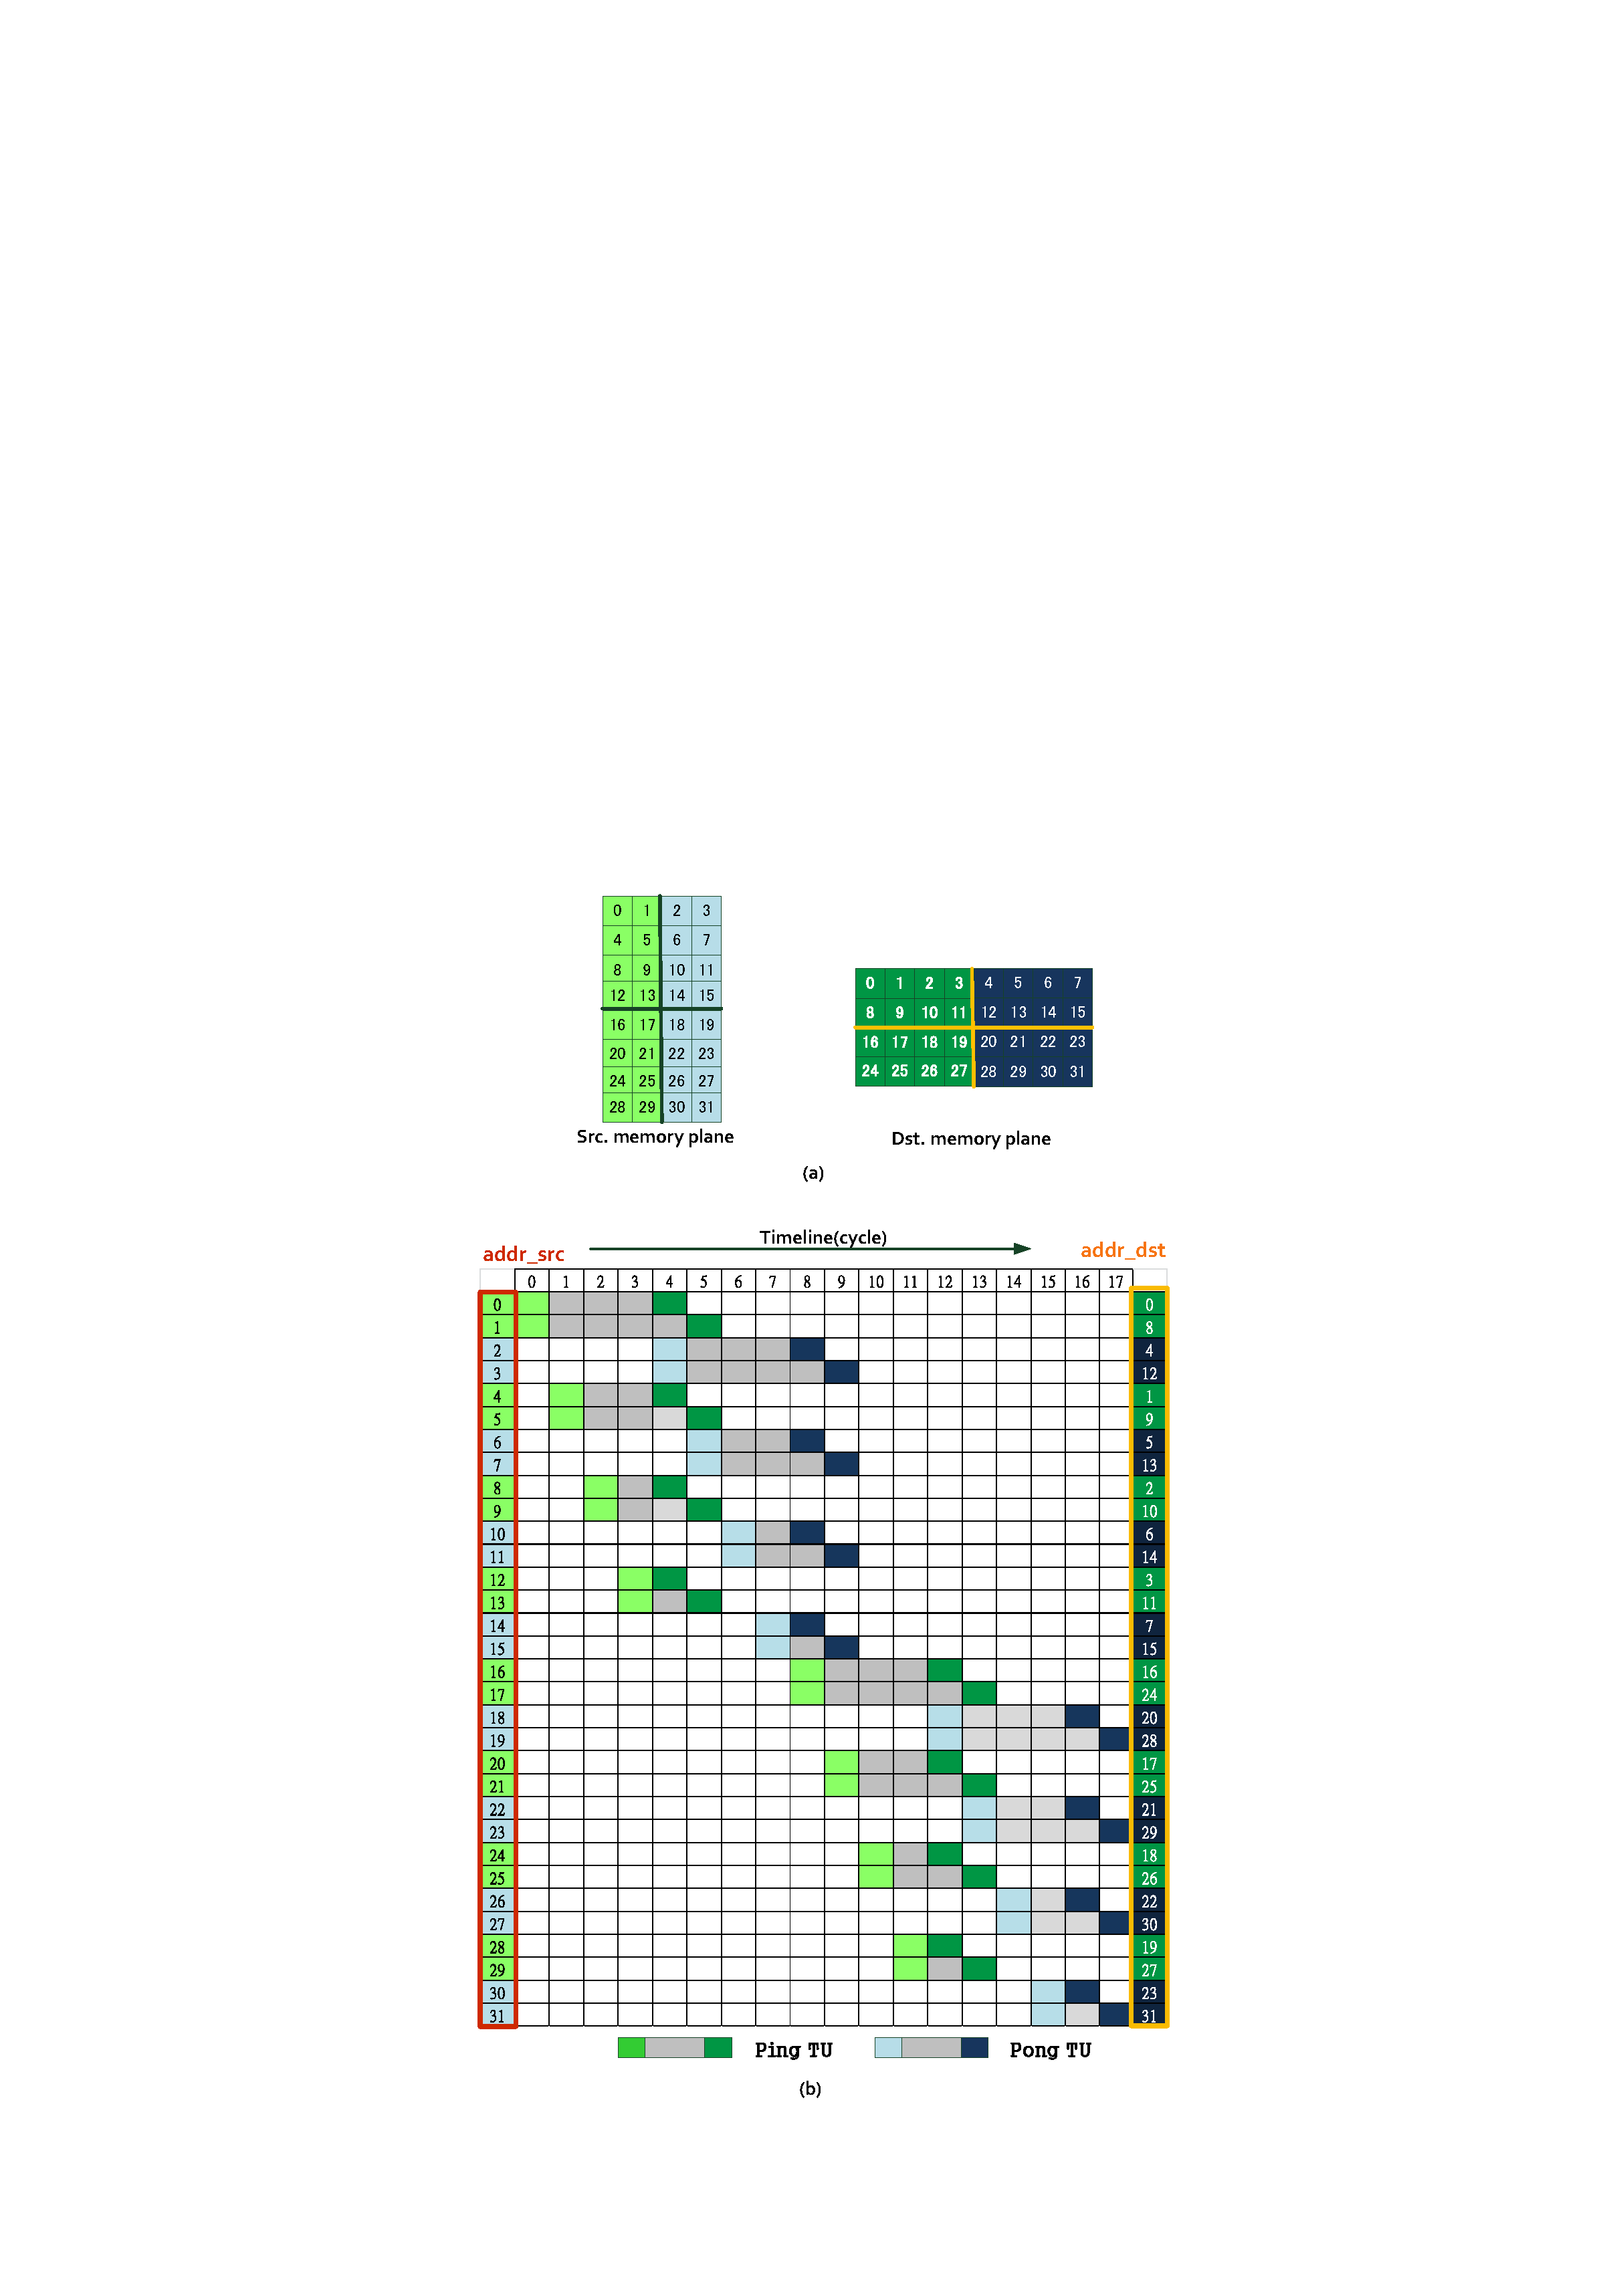
\includegraphics[scale=0.65]{Out_of_Order_Example_v03}
\caption{Out-of-order data motion between source memory and destination memory}
\label{fig:Out-of-Order_Example}
\end{center}
\end{figure}


\subsection{Finite State Machine }
While SC performs transpose, the control units would be in charge of control flow and data flow. State diagram of control units is shown in Figure \ref{fig:FSM}.
This FSM could be analyzed in two point of view.
First, we vertically cut this FSM.
LHS presents FSM of Ping TU, and RHS is FSM of Pong TU. These two FSMs coexist with dependence. Input/Output data from source satisfies single TU.
In this way, Ping and Pong alternately employ system bus. $ Done\_Iping $ and $  Done\_Ipong $ signals promise fluent data stream without conflict for source-side,
and $ Done\_Oping $ and $  Done\_Opong $ signals promise it for destination.

Second, we horizontally cut this FSM.
The upper part refers to importing form source, and the lower refers to exporting to destination. They have some properties in common. $ In\_Ping/$ $ In\_Pong $ is the state sending data from source memory into transpose unit ping/pong. In export FSM, likewise, $ Out\_Ping/$ $Out \_Pong $ is the state that data from transpose unit ping/pong retreats to GPU memory. They also need an address generator request to source and destination to generate coordinate addresses. However, the contract part of their behaviors is the timing for generating address to source or destination memory. In import state, control unit sends a load request to source memory, after read transaction, source memory outputs a burst of data to ping-pong transpose unit. In export state, the control unit sends a write request and generates output address to destination when ping-pong transpose unit outputs the data.

\begin{figure}[bt]
\begin{center}
\graphicspath{{picture/}}
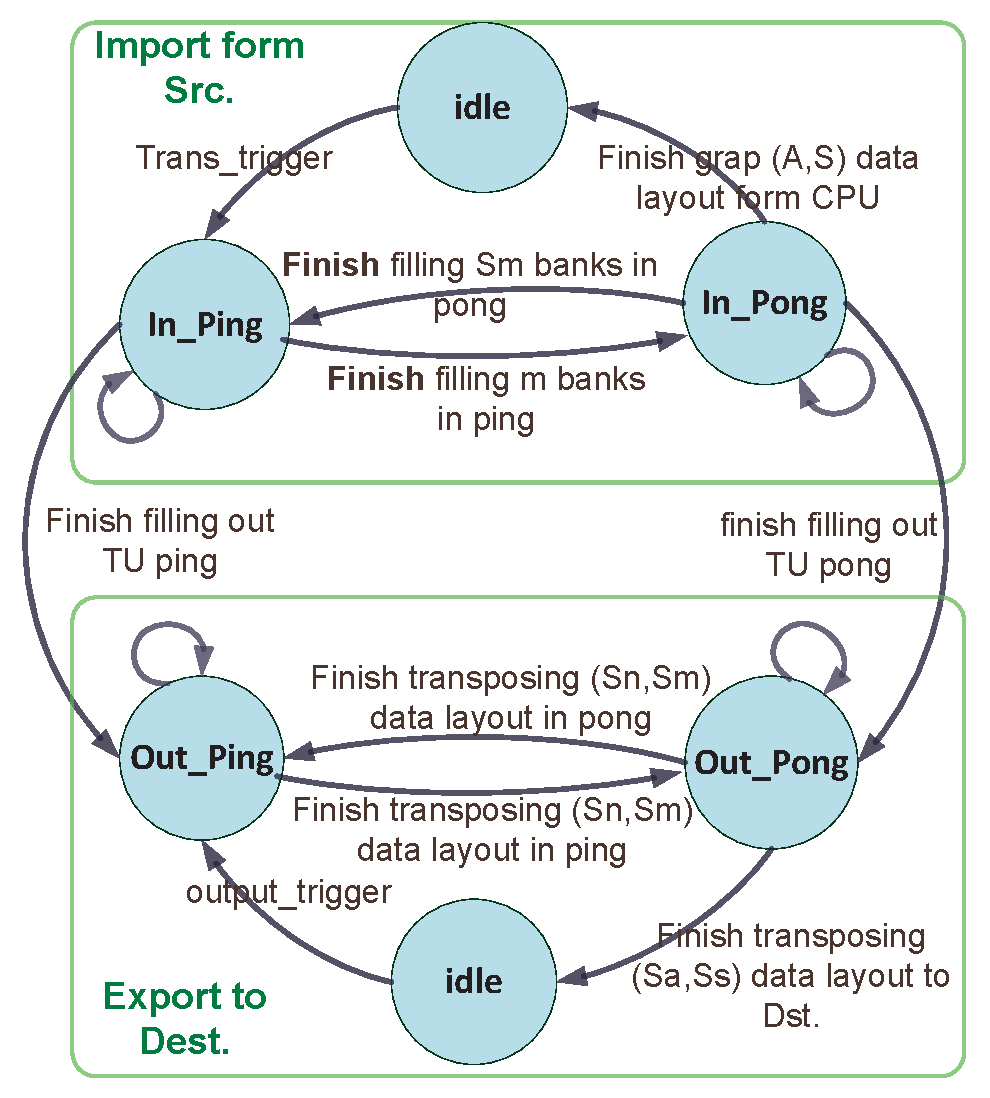
\includegraphics[scale=0.5]{FSM_v02}
\caption{Finite state machine of the system}
\label{fig:FSM}
\end{center}
\end{figure}






%===================================================
\section{Layout Conversion for Non Rectangular Patterns}\label{Special patterns}
In previous sections, we discuss the overall system architecture of proposed memory controller, which converts AOS layout to ASTA/SOA layout. However, our smart controller also supports lots of kinds of layout conversion: stride, diagonal, and sparse. In this section, we introduce the functions and the architecture of each converter.

%Such layout conversion can be defined as regular conversion because we convert entire layout with regular manner. However, in GPGPU computing, apart from regular conversion, we also need other kinds of layout converters to improve the performance of applications. In the follows, we introduce the irregular layout conversion.

\begin{algorithm} [h]
%\linesnumbered
%\scriptsize
%\footnotesize
\KwIn{
%$burst\_in $ is a continuous data accessed from source memory}
Parameters from memcpySC API}
\KwResult{
%$burst\_out $ is a continuous data that would be sent to destination memory}
Transformed data layout stores in the destination memory}
\Begin{
\If{Stride}{
    Stride-supported Transpose Unit();\\
	 Stride-supported Address Generator():\\
  }
 \If{Diagonal}{
	 Diagonal-supported Transpose Unit();\\
	 Diagonal-supported Address Generator():\\
  }
  \If{Sparse}{
                Histogram Unit();\\	
				ELL format Generator();\\
			    ELL format Generator();\\
  }
}
\caption{Advanced patterns()}
\label{alg:Advanced}
\end{algorithm}






\subsection{Stride Converter} \label{Stride}
Stride converter can gather the data with non-unit stride together. As showed in Figure \ref{fig:Stride}, begin with the $  start $ element, $ W0 $, then skip $ Stride $ elements to the  $ W1 $, over and over. The non-unit stride conversion can be formulated as $dest_layout=start+ stride \times i$. The destination data plane is a subset of the source data with a uniform stride. By remaining and gathering the useful data and discard the useful data, this kind of converter would benefit applications which only use a subset of the source data.

\begin{figure}[tpb]
\begin{center}
\graphicspath{{picture/}}
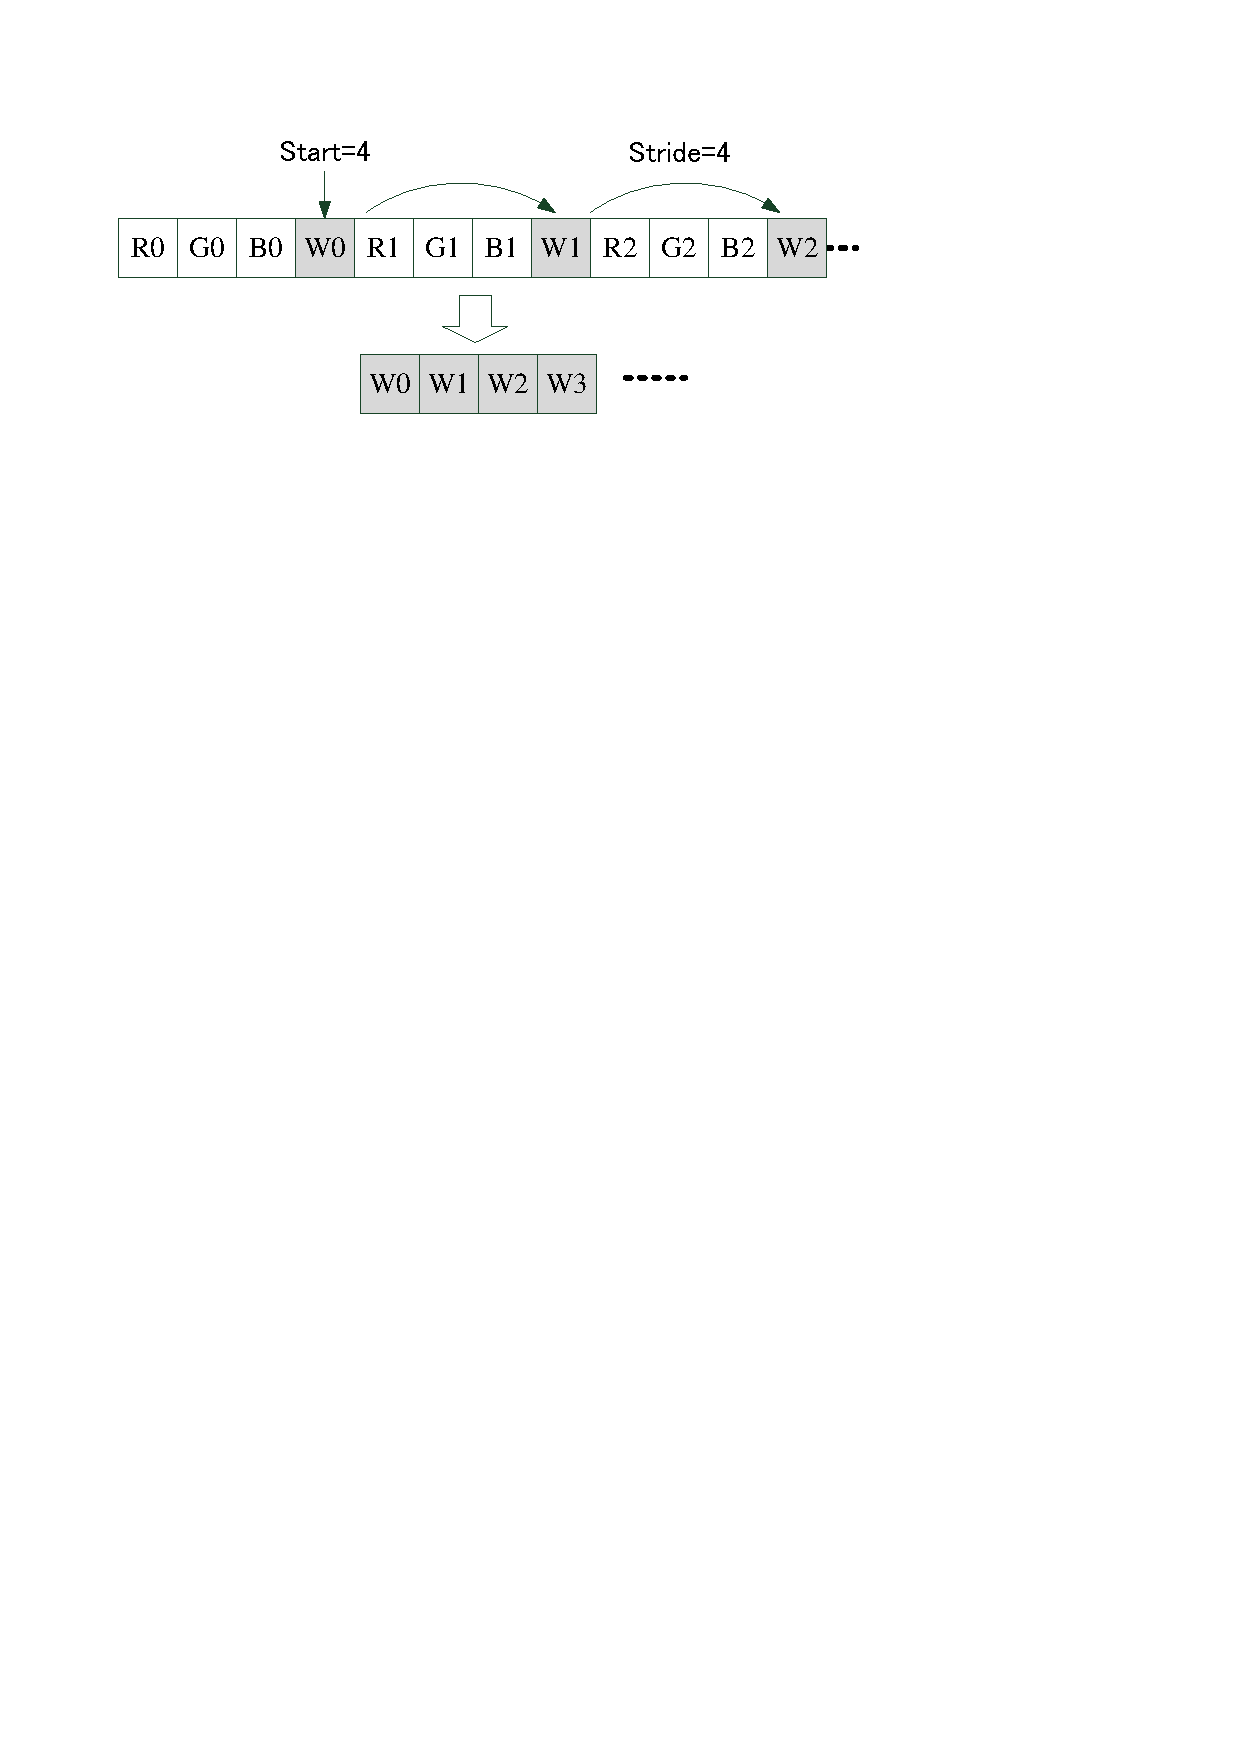
\includegraphics[scale=0.6]{stride}
\caption{An example of stride converter}
\label{fig:Stride}
\end{center}
\end{figure}


We take Viola-Jones based face detection \cite{facedetection} as example. The algorithm starts with Haar feature selection,
 calculating the intensity for each pixel by R, B, and G.
After the previous steps, we get the integral image. Sequentially, cascaded classifiers cooperating is used for classification. For the entire application, cascaded classification is the step which has the most significant amount of computations, and we find it only use integral image to compute instead of the RGB image. However, originally the storage of each pixel is R, G, B, and intensity, as shown in Figure \ref{fig:Stride}. Computing by this storage format would cause discontinuous memory access because the redundant R, G, and B. Therefore, stride converter gather intensities of each pixel together, and then the cascaded classifier can exploit this optimized data layout for calculation and gain the performance.

To allow the non-unit stride conversion, we only need to make slight modification to TU and AG. Conceptually, we can take the to-be-processed layout as AOS and then just output a subset of it.
The \textit{stride} can be regarded as $S_{s}$. The memory controller only output one data for every $S_{s}$.

For the part of AG, it doesn't need to traverse and process each data, instead, AG can jump into the end of each row because that is where the required data at.

On the other hand, we adjust the multiplexer of the TU. Instead of output data each cycle, the adjusted TU only output when necessary, that is, the last cycle for each round.




\subsection{Diagonal Converter}\label{Diagonal}

Proposed memory controller also support diagonal data layout conversion. Diagonal layout conversion means turning data layout with 45 degrees, as shown in Figure  \ref{fig:DiaExample} (b). This kind of conversion is needed when programmers want to improve the performance of   dynamic programming on GPUs. To maximize the thread level parallelism, dynamic programming usually be executed in diagonal manner. However, accessing data diagonally in data plane leads to poor data locality and even degrade the performance.
Therefore, we design a diagonal converter, which converts data in diagonal manner, and helps to coalesce data access for dynamic programming.
 For example, the Needleman-Wunsch \cite{NW} is a famous genetic alignment algorithm, which uses dynamic programming to compare biological sequences.
 Firstly, we model the problem by placing two DNA sequences in the first row and first column of the matrix. Next, initialize the matrix in the second row and second column. Then, score each cells from top-left to bottom-right, as shown in Figure \ref{fig:DiaExample} (a). When  executing on GPUs, cells on the same diagonal line can be parallel calculated by threads. However, this kind of calculation leads to poor data locality. As shown in Figure \ref{fig:DiaExample} (b), the colors mean the execution orders. We find that the cells executed in the same order are placed diagonally. To enhance the data locality, we convert the data layout so the data access in the same executing order becomes continuous. The diagonal converter therefore enhance the performance for dynamic programming.

%  the algorithm iterates over the whole matrix as well as fill it out with scores, traversing the matrix from left-top to right-bottom with "diagonal-strip" which leads to non-coalescing access. Such scheme, also known as Diagonal Strip Data Layout (DSDL), could not be converted efficiently by GPU kernels because it involves with complicated address mapping. As a result, the state-of-art solution, Dymaxion API \cite{Dymaxion}, only speedups the Needleman-Wunsch in Rodinia's GPU benchmark \cite{rodinia} by 1.2 times on average.



\begin{figure}[tpb]
\begin{center}
\graphicspath{{picture/}}
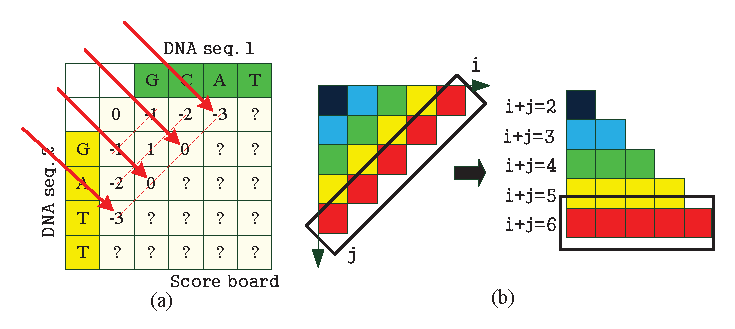
\includegraphics[scale=0.65]{Dia_Example}
\caption{An example of (a)Needleman-Wunsch (b) Diagonal Matrix}
\label{fig:DiaExample}
\end{center}
\end{figure}

%\subsubsection{Diagonal-supported Transpose Unit}
To support DSDL optimization, we extent TU by integrating the memory bank with a barrel shifter and thus burst data could be rotated to meet the requirement of the destination layout. More over, a selecting signal indicates which bytes could be written to the destination memory space. With such an extension, the executing flow of converting DSDL block by TU is shown in Figure.\ref{fig:Diagonal_TU}. Firstly, row by row burst data from the the non-coalescing layout is filled into the memory bank with particular rotation to coalesce vertically, as shown in Figure.\ref{fig:Diagonal_TU}(a). After the bank is filled, TU fetches the memory bank column by column and select specific bytes to generate coalescing burst data. Each block processed by TU becomes a coalescing diamond, as shown in Figure.\ref{fig:Diagonal_TU}(b).

\begin{figure}[t]
\begin{center}
\graphicspath{{picture/}}

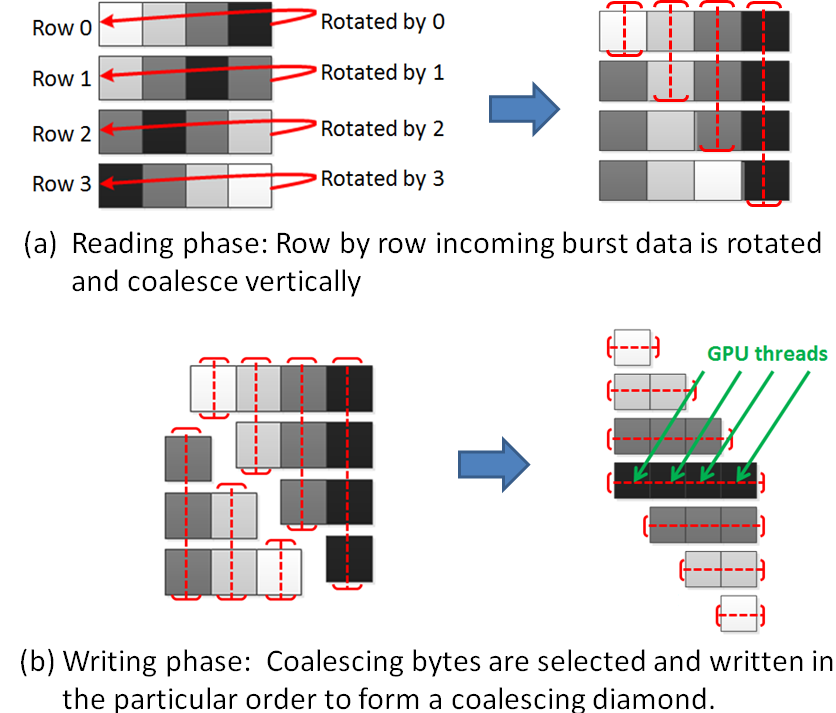
\includegraphics[scale=0.33]{tunewnew}

\caption{Execution flow of diagonal-supported TU}
\label{fig:Diagonal_TU}
\end{center}
\end{figure}

\begin{figure}[t]
\begin{center}
\graphicspath{{picture/}}

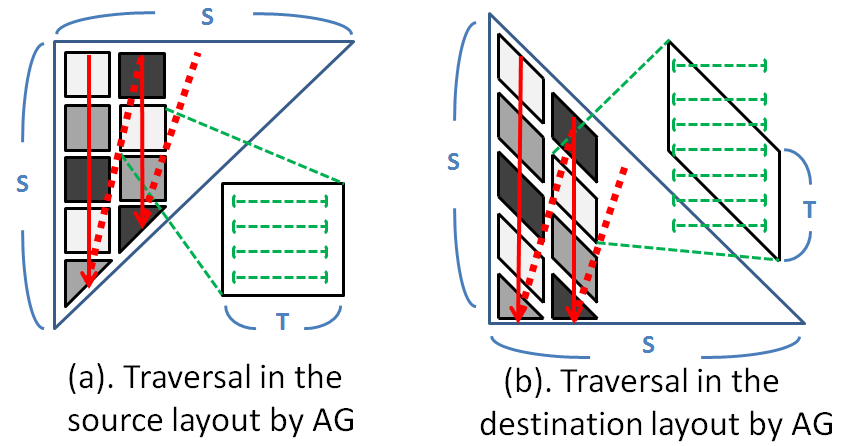
\includegraphics[scale=0.32]{agnew}

\caption{Layout traversal of diagonal-supported AG}
\label{fig:Diagonal_AG}
\end{center}
\end{figure}

%\subsubsection{Diagonal-supported Address Generator}

 %\indent An address generator (AG) is responsible for helping TU to assemble diamond blocks and form them into a completed layout, by determining addresses of source and destination for TU.
 The original design of AG includes an adder and basic control logics that perform address computing. As we extent AG to support DSDL conversion, a challenge emerged because DSDL conversion is involved with more complicated address calculation, which could degrade the throughput of the controller. \\
 \indent To eliminate address computing from the critical path, we simplify it by manipulating the symmetric property of DSDL, dividing it into upper-left and lower-right halves. The design of AG focuses on handling the upper-left half and the remaining could be completed in a symmetric approach. The execution of new AG is shown in Figure.\ref{fig:Diagonal_AG} and Algorithm.\ref{algo:DAG}. Let sizes of layout and TU be $S\times S$ and $T\times T$. By calculating the previous address plus $S$, AG traverses the layout in column major as well as generate a sequence of addresses sent to TU, completing a coalescing layout. Moreover, an address pre-fetch unit that buffers the first address in the next column is proposed, so complication of switching an address to a new column can be avoided. Let's demonstrate an example from a source layout. Suppose ${ADDR}_{i}$ and ${ADDR}_{j}$ are the first and last addresses of the same column respectively. Instead of calculating complicated ${ADDR}_{j+1}$ (i.e., the first address of the next column) based on ${ADDR}_{j}$, we pre-fetch it as soon as AG is iterating ${ADDR}_{i}$, by making use of the locality of two neighboring addresses.

\begin{algorithm}[tb]
\caption{Diagonal supported Address Generator}
%\scriptsize
\footnotesize
\label{algo:DAG}
%\end{center}
%\footnotesize
\textbf{Input:} $  S(layout~size), T(TU~size)$

\textbf{Output:} $ addr\_src$, and $addr\_dest $

%\textit{\textbf{In each cycle}}

% \Begin{	

            \ForEach{i=0 to $\frac{S}{T}-1$}
            {
                addr\_src = $i \times T$; \\
                \If {i==0}
                {
                    addr\_dst = $i \times T$; \\
                }
                \Else
                {
                    addr\_dst = read\_buffer(); \\
                }
                \ForEach{j=0 to $M - i\times T$}
                {
                    \If {$\frac{j}{T}$==i+1}
                    {
                        write\_buffer(addr\_dst+T); \\
                    }
                        output(addr\_src); \\
                        output(addr\_dst); \\
                        addr\_src += M; \\
                        addr\_dst += M; \\

                }

            }


\end{algorithm}


\subsection{Sparse Converter}\label{sparse}
We also devise a sparse matrix format converter.
%However, the default sparse format is Coordinate(COO).
The COO format is the most general format for the sparse matrix representation.
Many commercial libraries, such as Intel MKL \cite{Intel}, which supports
the matrix-vector multiplication for the sparse matrices in the COO format.
However, in parallel programing, the most efficient general sparse matrix format is ELL \cite{spmv_CUDA}.
To obtain better performance, programmers need a off-line transformation from COO to appropriate sparse format.
In order to reduce this overhead, our design automatically converts sparse data format from
COO to ELL during data copy duration.

Figure \ref{fig:SparseExample} illustrates an example to introduce these formats.
COO format intuitively stores both row and column index for each non-zero elements.
%Only non-zero elements are stored, and the coordinates of each non-zero element are given explicitly.
On the other hand, for ELL format, let $ K $ be the maximal number of non-zero elements among all rows;
for each row,  precisely $ K $ elements are stored (while the number of non-zero elements is less than $ K $,
extra zero value will be included). In more detail, ELL format stores not only element value but also the column index that is sorted by row index.
To sum up, we have COO format in source memory, containing value array ($ V_{COO} $), row array ($ R_{COO} $),
and column array ($ C_{COO} $) as the inputs. Each array contains $ N_{t} $ elements, where $ N_{t} $ presents the total non-zero elements.
After conversion, the targeting  ELL format in destination memory
may contain the value array($ V_{ELL} $), column array($ C_{ELL} $), and each array contains $ N_{r} \times K $ elements, where  $ N_{r}$
presents number of rows.
\begin{figure}[tpb]
\begin{center}
\graphicspath{{picture/}}
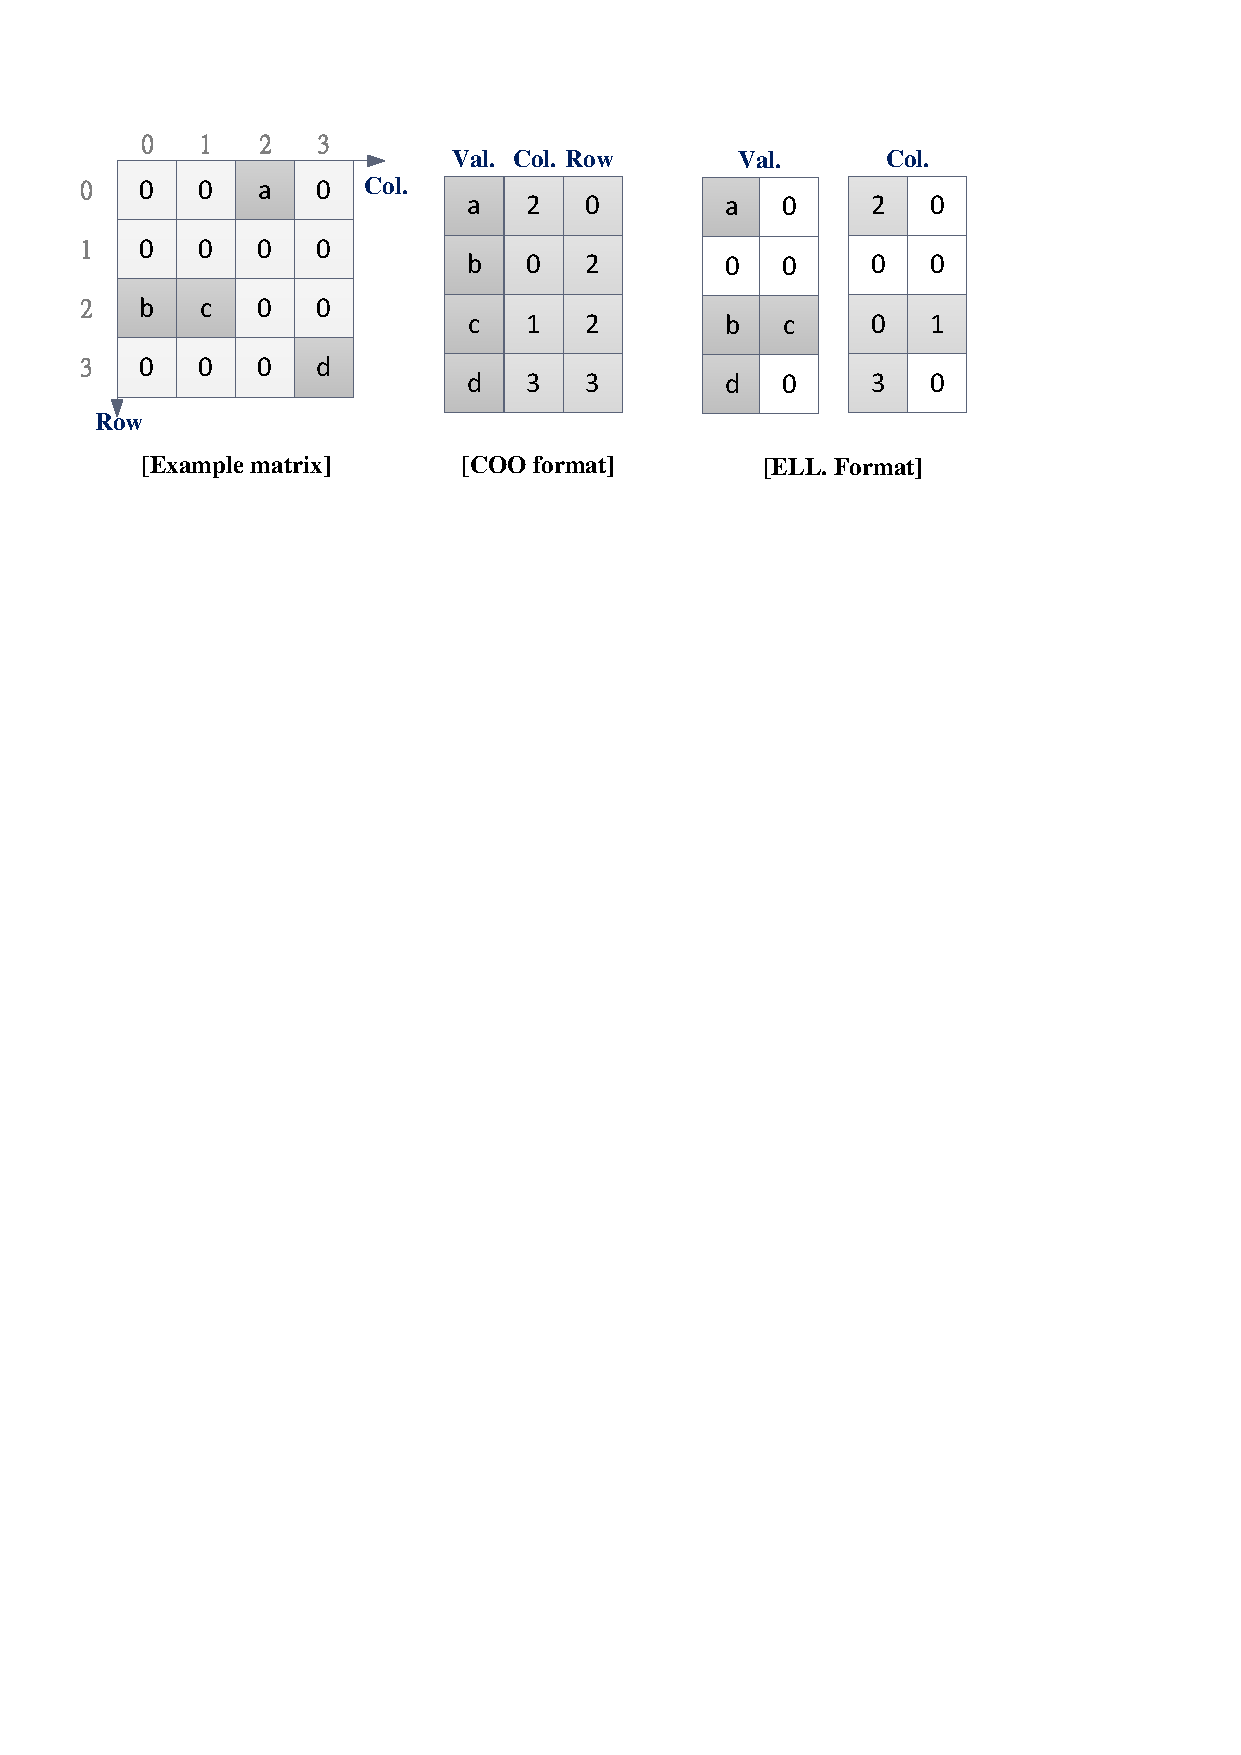
\includegraphics[scale=0.6]{SparseExample}
\caption{An example of sparse matrix format: COO and ELLPACK}
\label{fig:SparseExample}
\end{center}
\end{figure}

\subsubsection{Architecture of Sparse Converter}
To generate ELL format, the width of targeting array $ V_{ELL} $ and $ C_{ELL} $, the maximum number of non-zero elements $ K $, are needed to be determined in advance.
Thus, the first step of ELL format converter is to calculate the maximal number of non-zero elements, $ K $. Calculating $ K $
demands a histogram operation. The calculating algorithm and the modulation scheme is shown in Algorithm \ref{alg:Histogram}
and the upper part of Figure \ref{fig:ELL}.
Without storing the voting histogram array,
we present a deft and flexible circuit. Register $ target $ presents the target row, and, for each row, $ target\_counter $ calculate the number of non-zero elements for target row.
Register $ max $ is the temporary maximum number of non-zero elements.  The circuit inspect each input from $ R_{COO}[j] $.
When $target $ changes, current $ target\_counter $ presents the total non-zero number of last row. Then, comparing $ max $ with $ target\_counter $ to choose the relative maximum.

\begin{algorithm}  [t]
%\linesnumbered
%\scriptsize
\footnotesize
\KwIn{Row array of sparse matrix with COO format,  $ R_{COO}[j] $, where j=0,1,...,$ N_{t}   $
}

\KwResult{
Maximal number of non-zero elements among rows: $ K $
}

\Begin{
	target=0; target\_counter=0;	max=0;\\
  \For{$i\leftarrow 1$ \KwTo $  N_{t} $}{
  \If{$ R_{COO}[j] $=target}{
  	target\_counter++;
  }
  \ElseIf{$ R_{COO}[j] $  $>$target}{
  	target=$ R_{COO}[j] $;\\
  	\If{target\_counter $>$ max}{
  		max= target\_counter}
  	target\_counter reset to 1;
  }
  }
  }
\caption{Histogram Unit  }
\label{alg:Histogram}
\end{algorithm}


%ell format generator
%\subsection{ELL Format Generator}
After obtaining $ K $, two-dimension ELL arrays, $ C_{ELL}[i][j] $ and $ V_{ELL}[i][j] $, where i=0,1,...,$ N_{r}-1 $ and j=0,1,...,$  K-1 $, would be generated. Processing algorithm and circuits are shown in Algorithm \ref{alg:ELLFormat} and lower part of Figure \ref{fig:ELL}. Firstly, SC request destination memory to allocate two-dimension array with $N_{r}$ in height and $L$ in width, and the manager initials these arrays to be zero. Then, data with COO format would be send to exact position calculated by our mechanism, as shown in the algorithm.

Specially we notice about the zeros which is padded to the rows with less than $K$ non-zero elements.
%The main function of this block is not only mapping coordinate data from COO to ELL but also exactly padding zero to those non-stuffed ELL row.
To generate zeros in ELL, we have two choices: padding-during-process and pre-padding. Padding-during-process means the circuit sequentially fills value to $ C_{ELL}[i][j] $ and $ V_{ELL}[i][j] $ arrays, and the value contains both non-zero elements and zeros. Pre-padding means that two array $ C_{ELL}[i][j] $ and $ V_{ELL}[i][j] $ would be initialized to zero at beginning and then be filled with non-zero terms. While padding-during-process is a more institutive method, pre-padding improves 1\% to 48\% converting performance than padding-during-process depending on ELL density. Thus, we choose pre-padding as our zero processing strategy, and $ cudaMemset() $ is exploited to initialize array values.

\begin{algorithm}  [t]
%\linesnumbered
%\scriptsize
\footnotesize
\KwIn{Sparse matrix with COO-format, $  N_{t} $ is the total non-zero elements, L
}

\KwResult{
Sparse matrix with ELL-format stored in destination memory
}
\Begin{
 	allocate $C_{ELL} [N_{r}][L] $ and $V_{ELL} [N_{r}][L] $;\\
	initialize $C_{ELL}$ and  $V_{ELL}$ by cudaMemset(); \\
	target=0; target\_counter=0;	max=0;\\
  \If{R[j]=target}{
  	$ C_{COO} [j]  \rightarrow C_{ELL} [target][target\_counter] $;
  	$ V_{COO} [j]  \rightarrow V_{ELL} [target][target\_counter] $;
  	target\_counter++;\\
  }
  \ElseIf{R[j]>target}{
  	
  	target=R[j];\\	
  	target\_counter reset to 1;
  }
  }
\caption{ELL format Generator }
\label{alg:ELLFormat}
\end{algorithm}

\begin{figure}[t]
\begin{center}
\graphicspath{{picture/}}
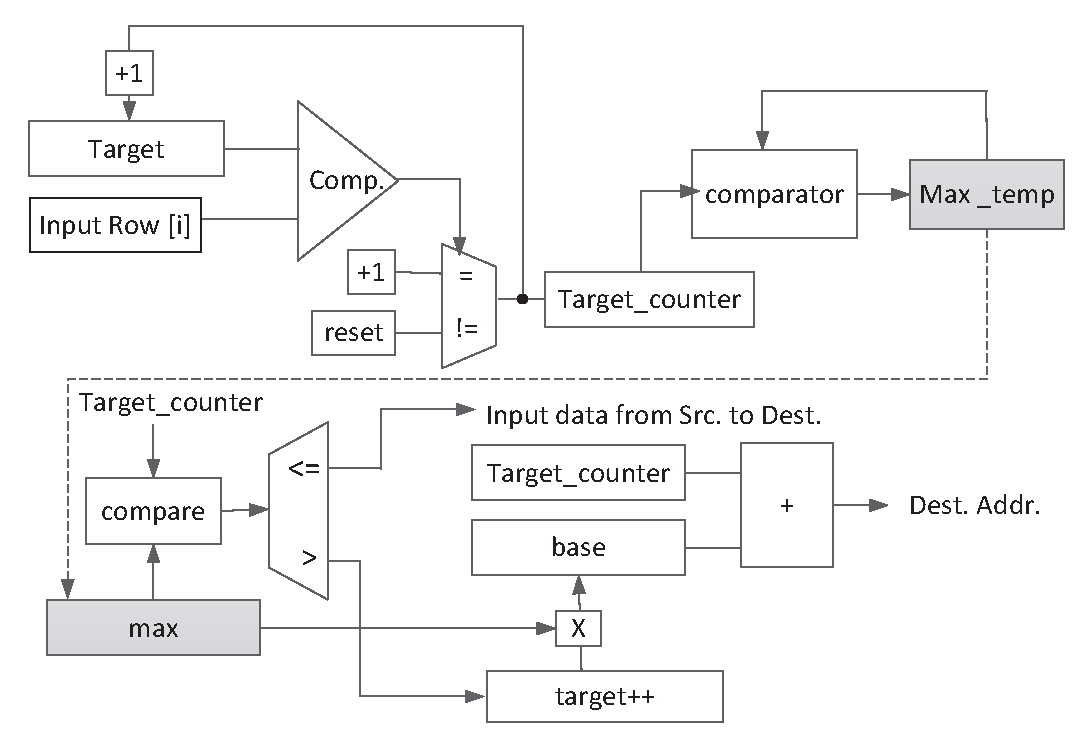
\includegraphics[scale=0.4]{ELL_generator}
\caption{Architecture of ELL format Generator Unit}
\label{fig:ELL}
\end{center}
\end{figure}




\section{Experiment}
\label{cha:experiment}
%==========environment~~~~
This section presents our experiments to demonstrate the capacities of the proposed memory manager.
Experiments were conducted on an NVIDIA GeForce 460 device and hosted in Intel Xeon E5420 CPU. We obtained GPU performance through the NVIDIA's CUDA profiler.
%==========================
%Equipped SC IP with CPU-GPU system, data layout marshaling on GPU would be more efficient.

We implement proposed circuits in Verilog and the synthesis details are shown in Table \ref{tb:synthesis}.
The memory manager is implemented by UMC 65nm CMOS technology with the maximum operating frequency at 1GHz.
Our design consumed 16,744 gate count and 0.3622 mW of dynamic power which is evaluated by Synopsys PrimeTime.

\subsection{Coalesced Transpose Evaluation}
In order to evaluate the efficiency of coalescing converter, we compared our design with the state-of-the-art software transpose library, PTTWAC\cite{ASTA}.
PTTWAC is an open-source library which implements the ASTA layout transformation. The post-synthesis simulation was adopted to
evaluate the performance of the proposed memory manager. In the experiment, host
and device memory hierarchy were simulated in test-bench and connected with gate-level manager architecture. The measurement of PTTWAC
library includes transfer and transpose time. The transfer time was measured by adopting our manager with normal mode, while
the transpose time was measured on NVIDIA GT460 GPU.

\begin{table}[]
\centering
\caption{Synthesis Results of Smart Controller}
\label{tb:synthesis}
\begin{tabular}{@{}
>{\columncolor[HTML]{FFFFFF}}l c@{}}
\toprule
Component               & Description \\ \midrule
Technology              & UMC 65nm    \\
Maximum frequency (GHz) & 1           \\
Power consumption(mW)   & 4.15        \\
Throughput(bits/cyc)    & 64          \\
Area(gate count)        & 20,093      \\ \bottomrule
\end{tabular}
\end{table}




\begin{table}[]
\renewcommand{\arraystretch}{1.2}
\centering
\caption{Description of benchmarks for the coalescing converter}
\label{tb:benchmarks}
\begin{tabular}{|c|c|c|c|c|}
\hline
Benchmark                                                                                       & Dataset                                                        & \begin{tabular}[c]{@{}c@{}}Row\\ (Node*)\end{tabular} & \begin{tabular}[c]{@{}c@{}}Column\\ (Dim*)\end{tabular} & \begin{tabular}[c]{@{}c@{}}Max.\# \\ nonzero\end{tabular} \\ \hline \hline
\multirow{3}{*}{\begin{tabular}[c]{@{}c@{}}Nearest\\ Neighbor*\end{tabular}}                    & Large                                                          & 131072                                                & 128                                                     & --                                                        \\
                                                                                                & Normal                                                         & 1024                                                  & 2048                                                    & --                                                        \\
                                                                                                & Small                                                          & 32                                                    & 32                                                      & --                                                        \\ \hline
\multirow{3}{*}{\begin{tabular}[c]{@{}c@{}}Matrix \\ Multiply\end{tabular}}                     & Large                                                          & 4096                                                  & 4096                                                    & --                                                        \\
                                                                                                & Normal                                                         & 1024                                                  & 1024                                                    & --                                                        \\
                                                                                                & Small                                                          & 63                                                    & 63                                                      & --                                                        \\ \hline
\multirow{3}{*}{Kmeans*}                                                                        & Large                                                          & 891                                                   & 2048                                                    & --                                                        \\
                                                                                                & \begin{tabular}[c]{@{}c@{}}Normal\\ (KDD cup)\end{tabular}     & 494020                                                & 36                                                      & --                                                        \\
                                                                                                & Small                                                          & 256                                                   & 256                                                     & --                                                        \\ \hline
\multirow{12}{*}{\begin{tabular}[c]{@{}c@{}}Spare \\ Matrix \\ Vector \\ Multiply\end{tabular}} & bcsstk18                                                       & 11948                                                 & 11948                                                   & 32                                                        \\
                                                                                                & e40r000                                                        & 17281                                                 & 17281                                                   & 62                                                        \\
                                                                                                & bcsstk31                                                       & 35588                                                 & 35588                                                   & 197                                                       \\
                                                                                                & bcsstk32                                                       & 44609                                                 & 44609                                                   & 215                                                       \\
                                                                                                & s3dkq4m2                                                       & 90449                                                 & 90449                                                   & 59                                                        \\
                                                                                                & \begin{tabular}[c]{@{}c@{}}conf6.0-0018\\ x8-8000\end{tabular} & 49152                                                 & 49152                                                   & 39                                                        \\
                                                                                                & cant                                                           & 62451                                                 & 62451                                                   & 78                                                        \\
                                                                                                & consph                                                         & 83334                                                 & 83334                                                   & 78                                                        \\
                                                                                                & cop20k\_A                                                      & 121192                                                & 121192                                                  & 81                                                        \\
                                                                                                & mac\_econ                                                      & 206500                                                & 506500                                                  & 44                                                        \\
                                                                                                & mc2depi                                                        & 525825                                                & 525825                                                  & 4                                                         \\
                                                                                                & pdb1HYS                                                        & 36417                                                 & 36417                                                   & 162                                                       \\ \hline
\end{tabular}
\end{table}

We evaluated four benchmarks, which
are nearest neighbor (NN), kmeans, matrix multiplication (MatMul), and sparse matrix vector multiplication (SpMV) with ELLPACK formats \cite{rodinia:}\cite{ASTA}\cite{AutoSpMV}. The data size of each benchmark is shown in Table \ref{tb:benchmarks}, and we evaluated each benchmarks with at least three data sets.
We measured the total transfer and transpose time of PTTWAC on NVIDIA GPU with 16, 32, and 64 tile size,
and we calculated the execution time of our SC coalescing converter.
The following Equation (\ref{t_convert_PTTWAC}) and Equation (\ref{t_convert_SC}) describe these two timing information, respectively.

\begin{align}
T_{conv}(PTTWAC)&= T_{transfer}(AOS_{CPU}\rightarrow AOS_{GPU}) \notag \\
&+ T_{PTTWAC}(AOS_{GPU}\rightarrow ASTA_{GPU}) \label{t_convert_PTTWAC}\\
T_{conv}(SC_{coalescing})&=
T_{SC}(AOS_{CPU}\rightarrow  ASTA_{GPU})  \label{t_convert_SC}
\end{align}
%===========

In Figure \ref{fig:transpose_benchmark}, we reveal the coalescing transformation speed up of SC over PTTWAC \cite{ASTA}.
%We take nearest neighbor(NN), kmeans, matrix multiply(MatMul) and sparse matrix vector multiplication(SpMV) as our benchmarks.
The result shows that, for the dense benchmarks, NN, MatMul, and kmeans, the manager performs
12.68 speed up than PTTWAC in average. Moreover, the manager performs best in NN by
 68.5 times, in MatMul by 35.35 times, and in kmeans by 52.63 times.
For the sparse benchmark, the manager performs
2.31 speed up than PTTWAC in average and performing best in mc2depi by 3.91 speed up with 16 tile size.

%For SpMV, we adopt 12 sparse matrices for transposing in ELLPCK format which is applied in \cite{ASTA}\cite{AutoSpMV}.
%The description of matrix is provided in table \ref{tb:SparseMatrix}, and the performance is shown in figure \ref{fig:transpose_SparseMatrix},
Compared to PTTWAC, transforming from AOS to ASTA layout with 16, 32, and 64 tile size, our design respectively achieves 4.38, 6.24 and 9.65 times speedup in average.
%This result shows the efficiency of our design in different dataset.
The proposed memory manager not only has the ability to reshape data layout but also capable to transfer data between host and device.
Thus, the current speedup is limited to the memory bandwidth for data motion, while it still performs significant speed up than state-of-the-art software solution.

\begin{figure*}[tb]
\begin{center}
\graphicspath{{picture/}}
%\scalebox{.9}{\includegraphics[width=\textwidth]{transpose_total}}
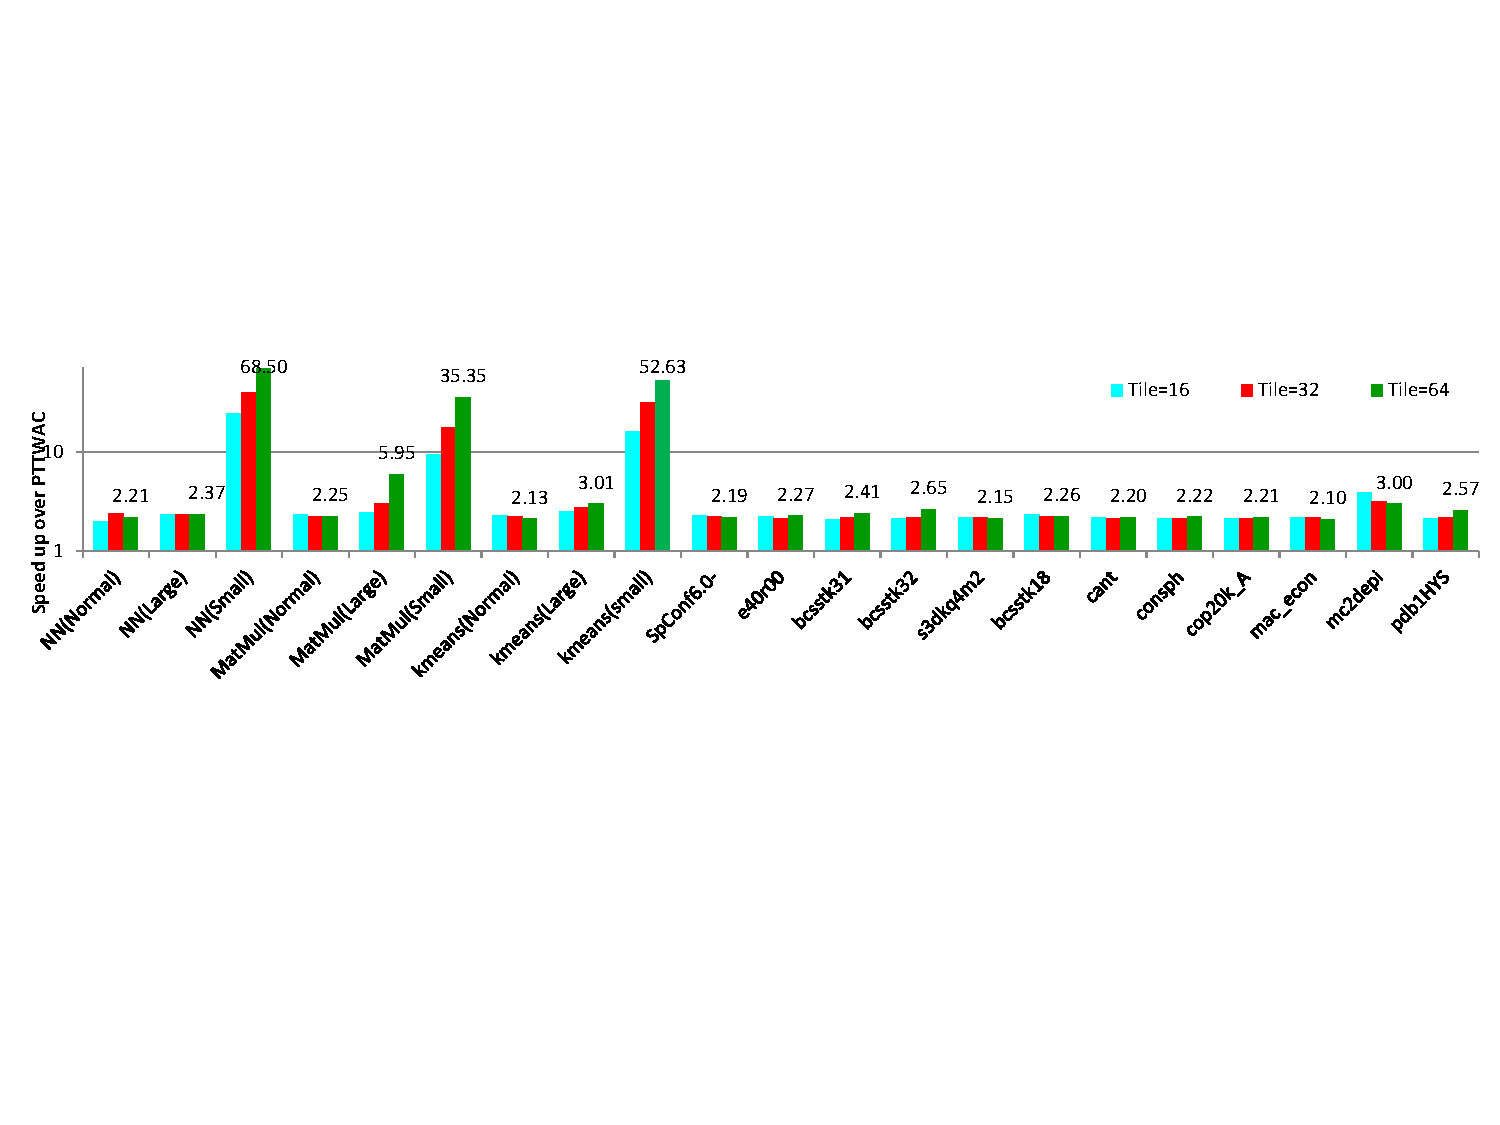
\includegraphics[width=\textwidth]{transpose_total_with_shape}
\caption{Data layout transpose and transferred timing comparison in each problem}
\label{fig:transpose_benchmark}
\end{center}
\end{figure*}


%------------overall evaluation-----------
\subsection{Application-level Analysis for Coalescing Converter}
In this subsection, we discuss the total execution time of the applications, including data movement, kernel execution times, and layout conversion latency.
As shown in Figure \ref{fig:OverallComputation}, for each benchmark, two kind of methods for optimizing layout, our memory manager and PTTWAC, are calculated in both kernel execution times and layout conversion latency, where the optimized layout is ASTA.
Moreover, kernel execution times of original layout without conversion is also listed.
The evaluated time of these three bars are formulated by Equation (\ref{t_total_original}-\ref{t_total_SC})

\begin{align}
\footnotesize
T_{total}(original)& =
 AOS_{CPU}\Rightarrow AOS_{GPU}\notag \\
 &+ execution(AOS) \label{t_total_original}\\
T_{total}(PTTWAC)&= T_{convert}(PTTWAC)  \notag \\
&+execution(ASTA) \label{t_total_PTTWAC}\\
T_{total}(SC_{coalescing})&=
 T_{convert}(SC_{coalescing})  \notag \\
& +\ execution(ASTA)  \label{t_total_SC}
\end{align}

To illustrate this figure, we take LHS of Figure \ref{fig:system} (d) as example. It is the SpMV application with data height 11948 and data width 32. For original scenario, data transfer from CPU to GPU spends 0.48ms and kernel execution  with AOS-type layout spensd 0.83 ms. For optimized by PTTWAC\cite{ASTA} scenario, data transfer spends 0.48 ms, layout conversion by software library spends 0.6 ms and kernel execution with ASTA-type layout spends 0.07 ms. For optimized by proposed SC scenario, SC combines data transfer and layout conversion into single step and it took 0.48 ms, and kernel execution with ASTA-type layout spends 0.07 ms.

We firstly discuss the kernel execution time of it. For each benchmark, kernel application with optimized data layout gets significant enhancement because of the improvement of DRAM efficiency. We illustrate the DRAM throughput in Table \ref{tb:DRAM_throughput}. In all benchmarks, SOA and ASTA layout perform much better than AOS in DRAM write throughput.
The significant performance improvement is explained by the fact that coalesced data layouts prevent the memory access processing from non-continuous accessing and contribute to improving the memory access efficiency in kernel execution.

Secondly, we consider the overall performance comparison.
For computation-bounded applications, such as NN and MatMul, adopting converted layout performs 3.33-12.20 times speed up.
For memory-bounded applications, such as kmeans and SpMV, because the data size of them are considerable,  therefore, layout conversion time of it is a huge overhead for entire applications. By SC, application-level performance of memory-bounded applications improves 2.13 times than original and  1.90 times than software method \cite{ASTA}.
%Clearly, reducing data transformation latency in memory-bounded application would significantly improve overall performance.

\begin{figure*}[tb]
\begin{center}
\graphicspath{{picture/}}
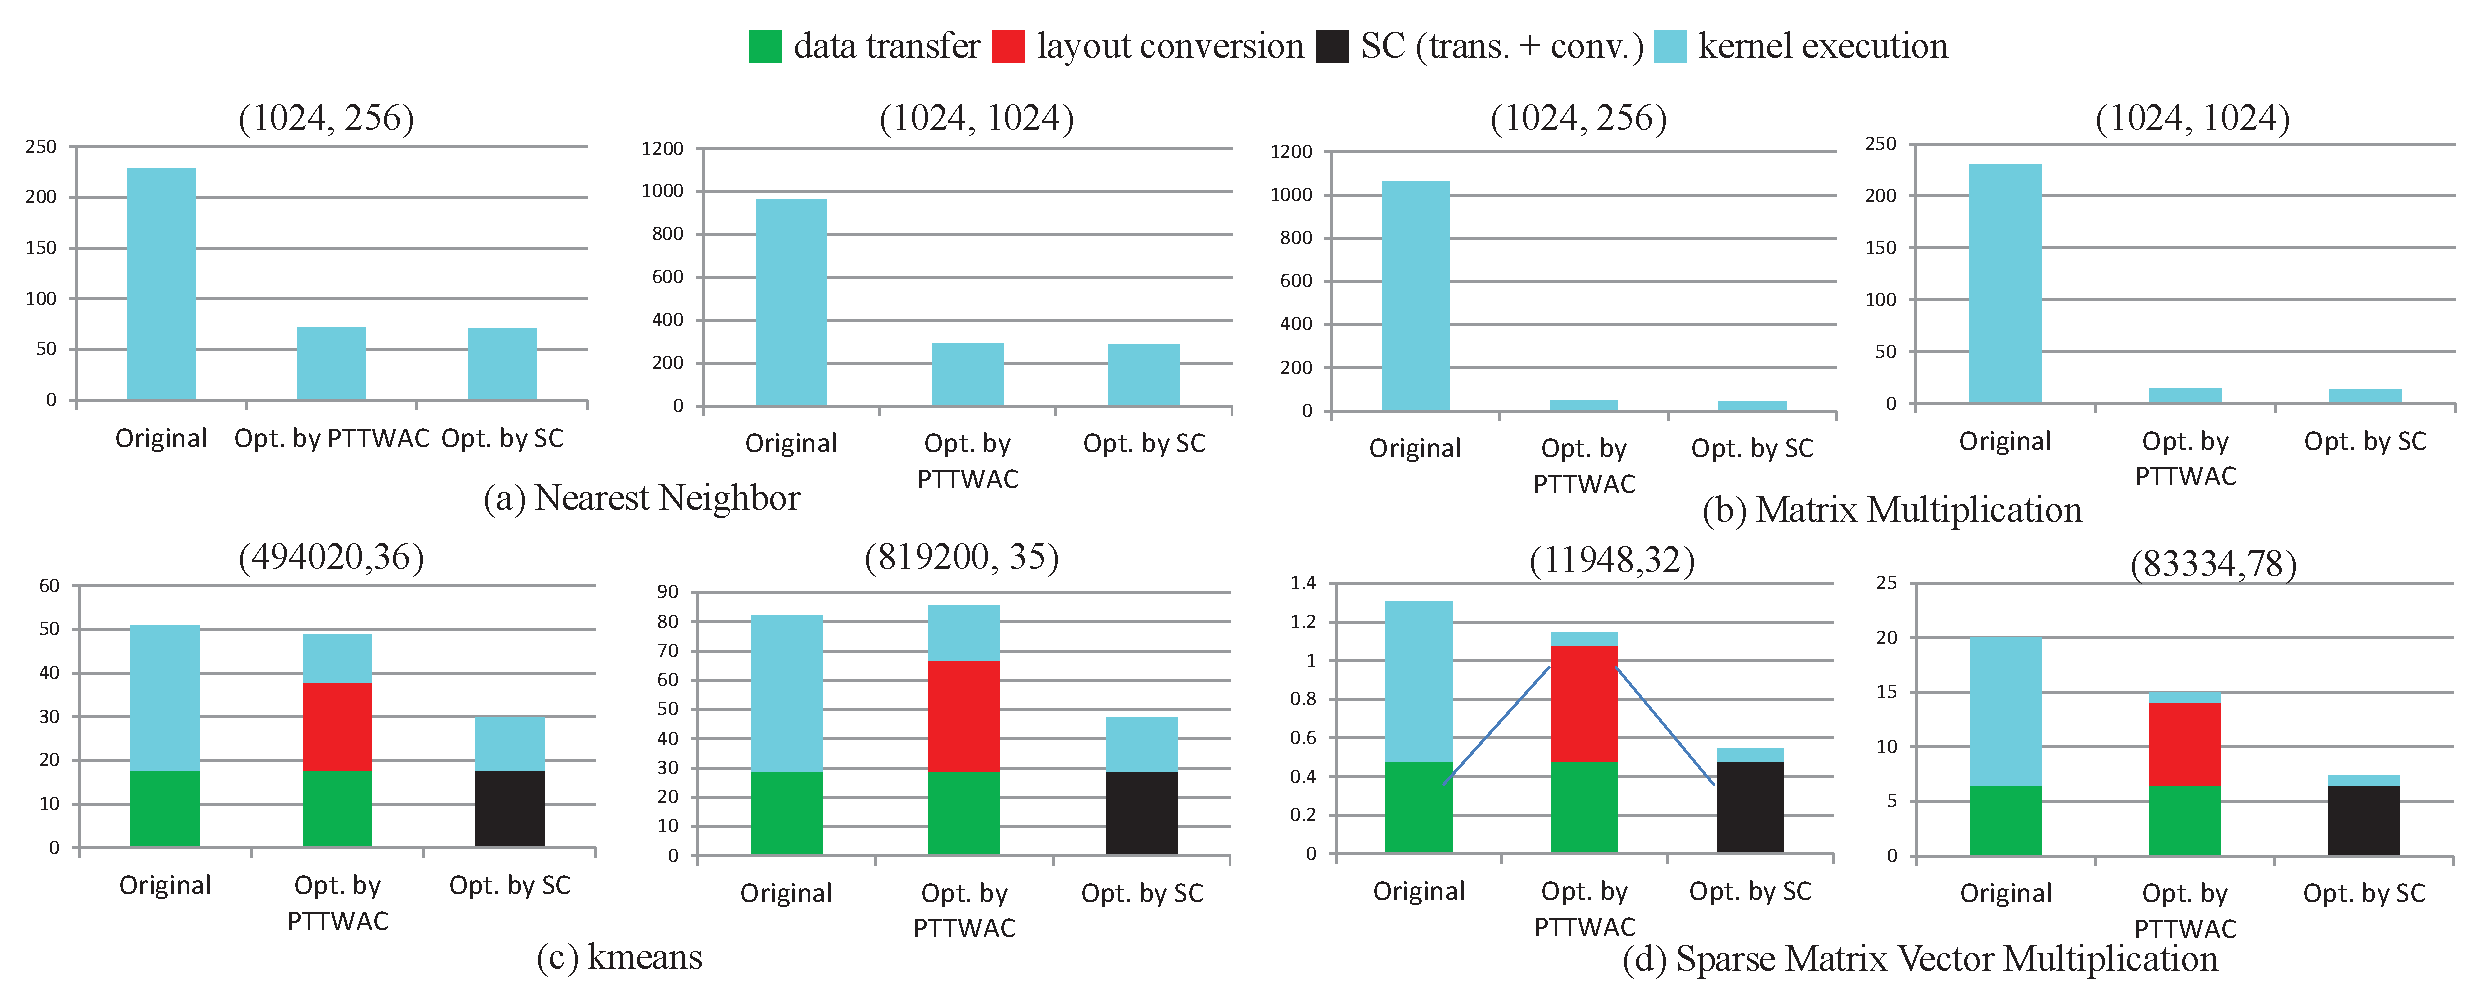
\includegraphics[width=\textwidth]{OverallComputation_06}
\caption{System-level performance(ms)(a)Nearest Neighbor (b)Matrix Multiplication (c) kmeans (d) sparse matrix vector multiplication }
\label{fig:OverallComputation}
\end{center}
\end{figure*}





\begin{table}[]
\renewcommand{\arraystretch}{1.3}
\centering
\caption{GPU DRAM throughput during kernel applications }
\label{tb:DRAM_throughput}
\begin{tabular}{|l|l|r|l|l|l|l|}
\hline
\multicolumn{1}{|c|}{\multirow{2}{*}{}} & \multicolumn{3}{l|}{Write Throughput (GB)} & \multicolumn{3}{l|}{Read Throughput (GB)} \\ \cline{2-7}
\multicolumn{1}{|c|}{}                  & AOS           & SOA          & ASTA        & AOS          & SOA          & ASTA        \\ \hline \hline
NN                                      & 0.0007        & 0.005        & 0.002       & 4.76         & 13.27        & 13.77       \\ \hline
MatMul                                  & 0.030         & 0.290        & 0.473       & 57.53        & 19.88        & 51.25       \\ \hline
kmeans                                  & 3.07          & 43.79        & 31.33       & 86.15        & 43.9         & 54.67       \\ \hline
SpMV                                    & 0.102         & 1.1          & 1.2         & 69.86        & 52.39        & 56.07       \\ \hline
\end{tabular}
\end{table}



\subsection{Analysis of Sparse Converter}
In previous subsections, we evaluate the sparse matrix transformation of ELLPACK from original to optimized ones, while in most scenario, sparse matrices are designed in COO format. In this section, we discuss the efficiency of our sparse converter, which performs a direct conversion from COO format to optimized ELL layout.
Our matrix suits are from \cite{matrix_market} which uses COO format with metadata as the default matrix representation.
The description of the tested matrices is shown in Table  \ref{tb:sparse_benchmark}.

We evaluated four scenarios for transferring data from host (CPU) to device (GPU) and layout conversion from $ COO $ to $ ELL_{SOA} $, including
%PTTWAC\cite{ASTA} with preprocessing($ T_{COO\rightarrow ELL, conv}(PTTWAC)$), coalescing converter with preprocessing($ T_{COO\rightarrow ELL, conv}(SC_{coalescing})$), cusp($ T_{COO\rightarrow ELL, conv}(cusp)$), and sparse converter($ T_{COO\rightarrow ELL, conv}(SC_{sparse})$)
PTTWAC with software-based preprocessing, coalescing converter with software-based preprocessing, software-based library CUSP \cite{Cusp}, and our sparse converter.
%The source layout is $ COO $, and the target layout is $ ELL_{SOA} $
Both PTTWAC and coalescing converter only address transformation from AOS-type to SOA-type layout; therefore extra software-based preprocessing is required for turning $ COO $ to $ ELL_{AOS} $ before transferring to GPU.
CUSP is a software-based library that supports data format conversion for sparse matrix.
%then turning $ ELL_{AOS}$ to $ ELL_{SOA}$.
%While cusp and  $ SC_{sparse}$ directly transpose from $ COO $ to $ ELL_{SOA} $.
The timing measurement includes both data motion and layout conversion.
%We measure converter performs both data motion and layout conversion, and we formulate
The execution time of the four scenarios can be decomposed into Equation (\ref{T1}) to (\ref{T4}), respectively.
The experimental result is illustrated in Figure \ref{fig:sparse_total_performance}. We took PTTWAC with software-based preprocessing ($T_{1} $) as the baseline.
%and evaluate the speed up of other 3 scenario ($T_{2}-T_{4} $) over it.
As the software-based preprocessing is conducted by CPU, which resulted in tremendous transpose overhead.
Our sparse converter directly reshapes $ COO $ to $ ELL_{SOA} $ format when data motions between CPU-GPU depending on a deft hardware design, and it achieves 2.71 times speedup than CUSP in average and about
362.29 times speed up than PTTWAC/SC with software-based preprocessing.

\begin{align}
\footnotesize
 T_{1}& =
  T_{CUSP}(COO_{CPU}\rightarrow ELL_{CPU,AOS})\notag \\
  &+ T_{transfer}(ELL_{CPU,AOS}\rightarrow ELL_{GPU,AOS}) \notag \\
  &+ T_{PTTWAC}(ELL_{GPU,AOS}\rightarrow ELL_{GPU,SOA})
  \label{T1}\\
 T_{2}& =
  T_{CUSP}(COO_{CPU}\rightarrow ELL_{CPU,AOS})\notag \\
  &+ T_{SC_{coalescing}}(ELL_{CPU,AOS}\rightarrow ELL_{GPU,SOA})
  \label{T2}\\
  T_{3}& =
  T_{transfer}(COO_{CPU}\rightarrow COO_{GPU}) \notag \\
  &+ T_{CUSP}(COO_{GPU}\rightarrow ELL_{GPU,SOA})
    \label{T3}\\
  T_{4}& =
  T_{SC_{sparse}}(COO_{CPU}\rightarrow ELL_{GPU,SOA})
   \label{T4}
 \end{align}



\begin{table}[]
\renewcommand{\arraystretch}{1.2}
\centering
\caption{Sparse matrix test suit}
\label{tb:sparse_benchmark}
\begin{tabular}{lrrcll}
\hline
\multicolumn{1}{c}{Dataset} & \multicolumn{1}{c}{\begin{tabular}[c]{@{}c@{}}Row/\\ Col\end{tabular}} & \multicolumn{1}{c}{\begin{tabular}[c]{@{}c@{}}Total \\ non-zero\\ elements\end{tabular}} & \begin{tabular}[c]{@{}c@{}}Max\\ non-zero\\ per row\end{tabular} & \multicolumn{1}{c}{\begin{tabular}[c]{@{}c@{}}Orig. \\ dens.\end{tabular}} & \multicolumn{1}{c}{\begin{tabular}[c]{@{}c@{}}ELL \\ dens.\end{tabular}} \\ \hline \hline
Bcsstk18                    & 11,948                                                                 & 149,090                                                                                  & 32                                                               & 0.00104                                                                    & 0.38995                                                                  \\ \hline
pdb1HYS                     & 36,417                                                                 & 4,344,765                                                                                & 162                                                              & 0.00328                                                                    & 0.73646                                                                  \\ \hline
mc2depi                     & 525,825                                                                & 2,100,225                                                                                & 4                                                                & 0.00001                                                                    & 0.99854                                                                  \\ \hline
qcd5\_4                     & 49,152                                                                 & 1,916,928                                                                                & 39                                                               & 0.00079                                                                    & 1                                                                        \\ \hline
consph                      & 83,334                                                                 & 6,010,480                                                                                & 78                                                               & 0.00087                                                                    & 0.92469                                                                  \\ \hline
rma10                       & 46,835                                                                 & 2,374,001                                                                                & 145                                                              & 0.00108                                                                    & 0.34958                                                                  \\ \hline
\end{tabular}
\end{table}


 \begin{figure}[tb]
 \begin{center}
 \graphicspath{{picture/}}
 %\includegraphics[scale=0.3]{transpose_Matrix}
 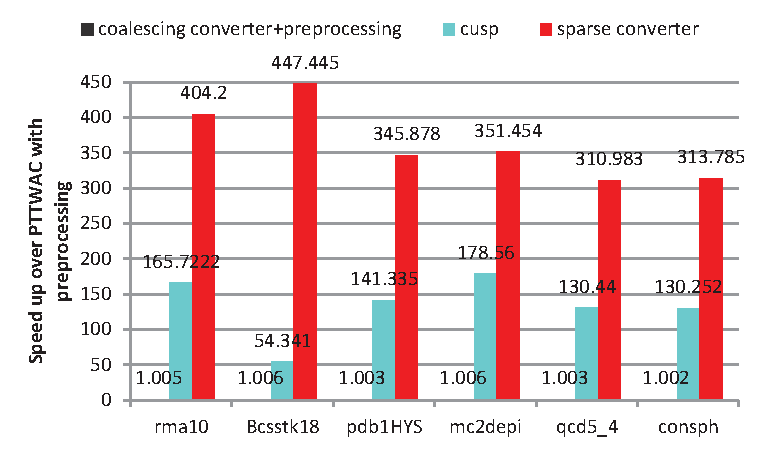
\includegraphics[scale=0.6]{sparse_COOtoELL_total}
 \caption{Performance comparison of sparse format conversion($ COO $ to $ ELL_{SOA} $) }
 \label{fig:sparse_total_performance}
 \end{center}
 \end{figure}

\subsection{Performance of Diagonal Converter}
In this subsection, we show the performance of diagonal converter.
As shown in Figure \ref{fig:Dia_performance}, we evaluated various DP benchmark programs, Needleman-Wunsch (NW), Minimum cost path (MCP) and Knapsack problem (KP) featuring DSDL. The problem size of these three problems vary from $128^2$ to $1024^2$. We calculate the time period from data transferring  to completing the problem in three scenario: Original, optimized layout by GPU, and optimized layout by proposed smart controller. The evaluated time of these three bar are similar to Equation (\ref{t_total_original}-\ref{t_total_SC}).



%We optimized memory layouts in both software and proposed hardware-based approaches that are both compared with original programs without any optimization. Details of the software-based approach, Dymaxion API, could be seen in \cite{Dymaxion}. Our evaluation of original DP programs including data transfer between CPU/GPU and GPU kernel execution. Furthermore, the legend of "GPU layout conversion" represent the extra burden on optimizing data layout of GPU and "HW transfer+conversion" is the layout conversion overlapped with transfer time by the hardware. The problem size varied from $128^2$ to $1024^2$ and execution time was measured in micro-second. \\
\indent By layout conversion, the GPU kernel execution time of NW, MCP and KP gained 4.9 to 2.1 times speedup over four problem sizes, as shown in the blue bars. Either software-based solution or our smart controller can  achieve these improvement.

However, if we take conversion time into account, the efficiency of software-based solution is not good, that means, converting a layout to diagonal-shape in GPUs is inefficient   because it suffered from the non-coalesced access when converting. Therefore, the overall performance of software-based solution is around  1.13 to 1.04 times speedup over the original cases. Our hardware, on the other hand, benefited from high throughput that overlap layout conversion with data transfer. Since the conversion overhead was hidden, it overall achieved 2.9 to 1.8 times speedup, and outperformed the solution of software-based conversion by 2.6 to 1.7 times speedup.% To sum up, our memory controller outperform the software-based API and bring significant improvement on DSDL programs across different problem sizes.


\begin{figure*}[t]
 \begin{center}
 \graphicspath{{picture/}}
 %\scalebox{.9}{\includegraphics[width=\textwidth]{transpose_total}}
 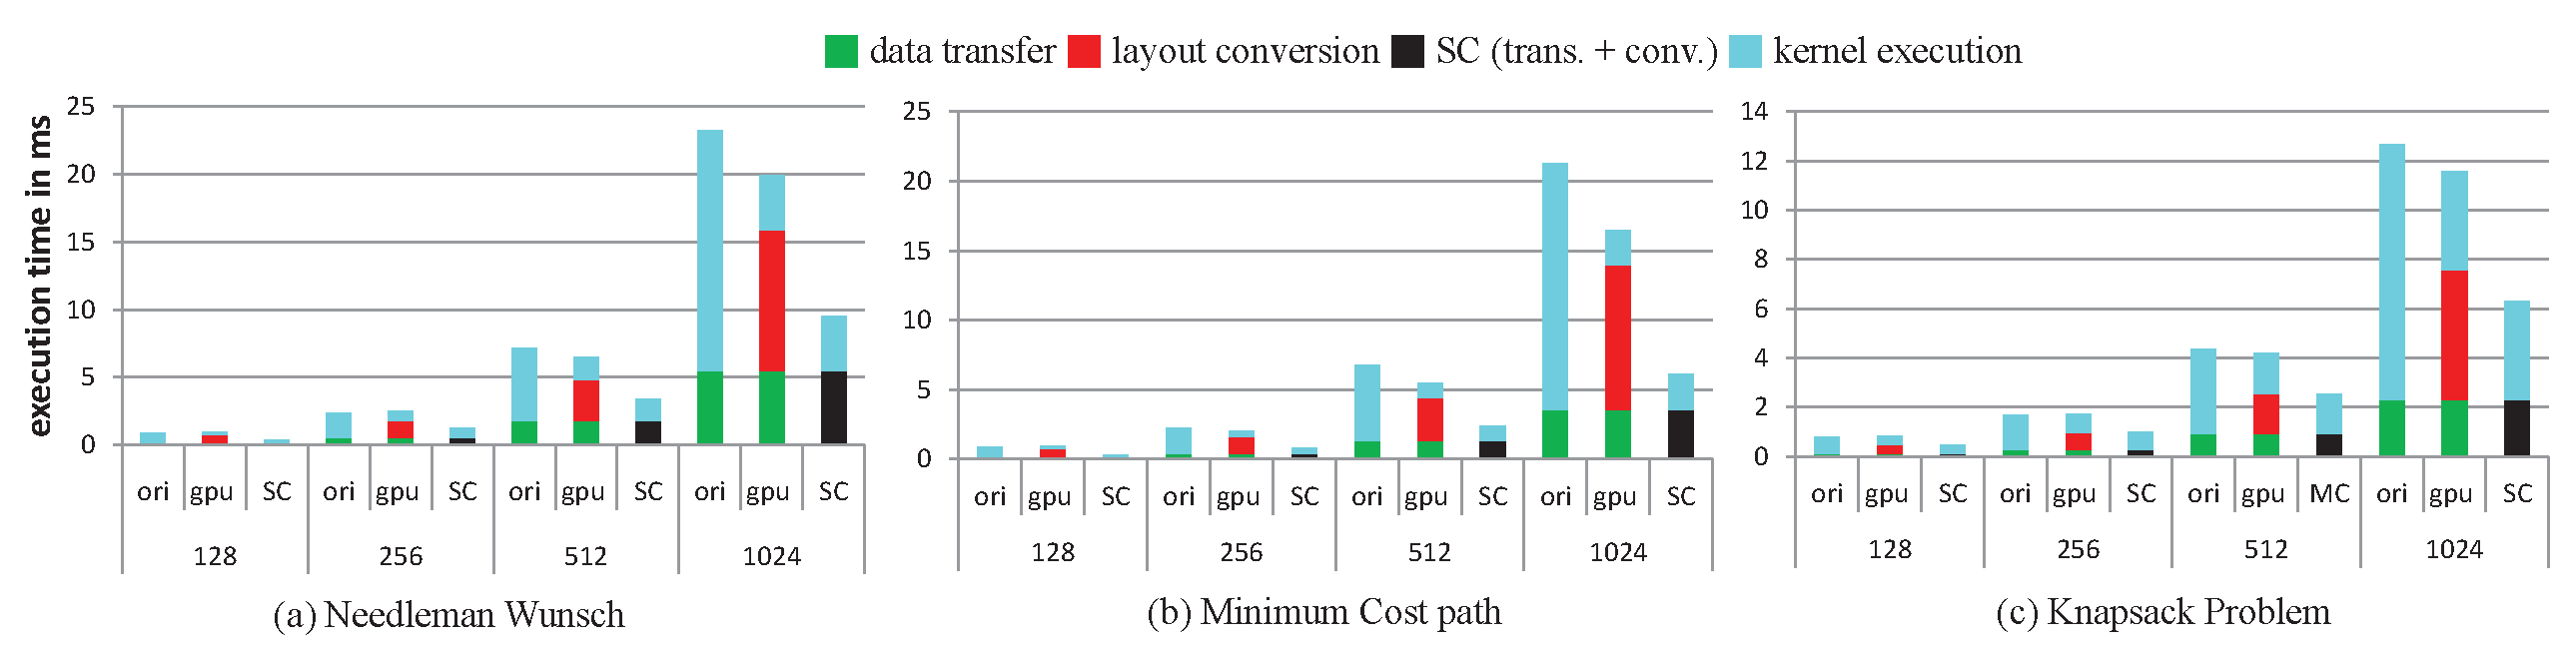
\includegraphics[scale=0.42]{Dia_experiment}
 \caption{Improvement on DSDL applications}
 \label{fig:Dia_performance}
 \end{center}
 \end{figure*}


\subsection{Performance of Stride Converter}
In this section, we present the experimental result of stride converter. We take the Haar face detection application as an example with an input image which is 4096x1080 in size. The experiment framework is based on OpenCL and both CPU and GPU are chosen as computing devices separately. As mentioned in section 4.1. Haar face detection is one of image processing applications that demand only the W channel (intensity). Consequently, both CPU and GPU could suffer from non-coalescing data access because there are always redundant RGB data between neighboring intensity information. By proposed stride converter, such scenario could be avoided by rejecting redundancy and aligning useful data  during data transfer.

\indent As shown in Figure. 17, the kernel execution time of Haar face detection achieves 2.02 and 1.52 times on CPU and GPU respectively with stride conversion. Looking into two stages, Cascaded Classifiers and Integral Image of the application, one could notice that there is 3 times speed-up on CPU in the former, which implies the data coalescing issue is the main bottleneck of CPU in this stage. Integral image, which demands massive computation, only gains 1.28 times speedup on CPU because the bottleneck lies on lack of computation power rather than data locality. GPU, on the other hand, gains about 1.5 times speedup evenly in both phases. Note that the proportion of Integral Image in kernel execution time on GPU is much less than on CPU, because this stage can be parallelized easily. To sum up, stride conversion improves performance of both CPU and GPU, as well as save the destination memory space by 75\%

 \begin{figure}[tb]
 \begin{center}
 \graphicspath{{picture/}}
 %\includegraphics[scale=0.3]{transpose_Matrix}
 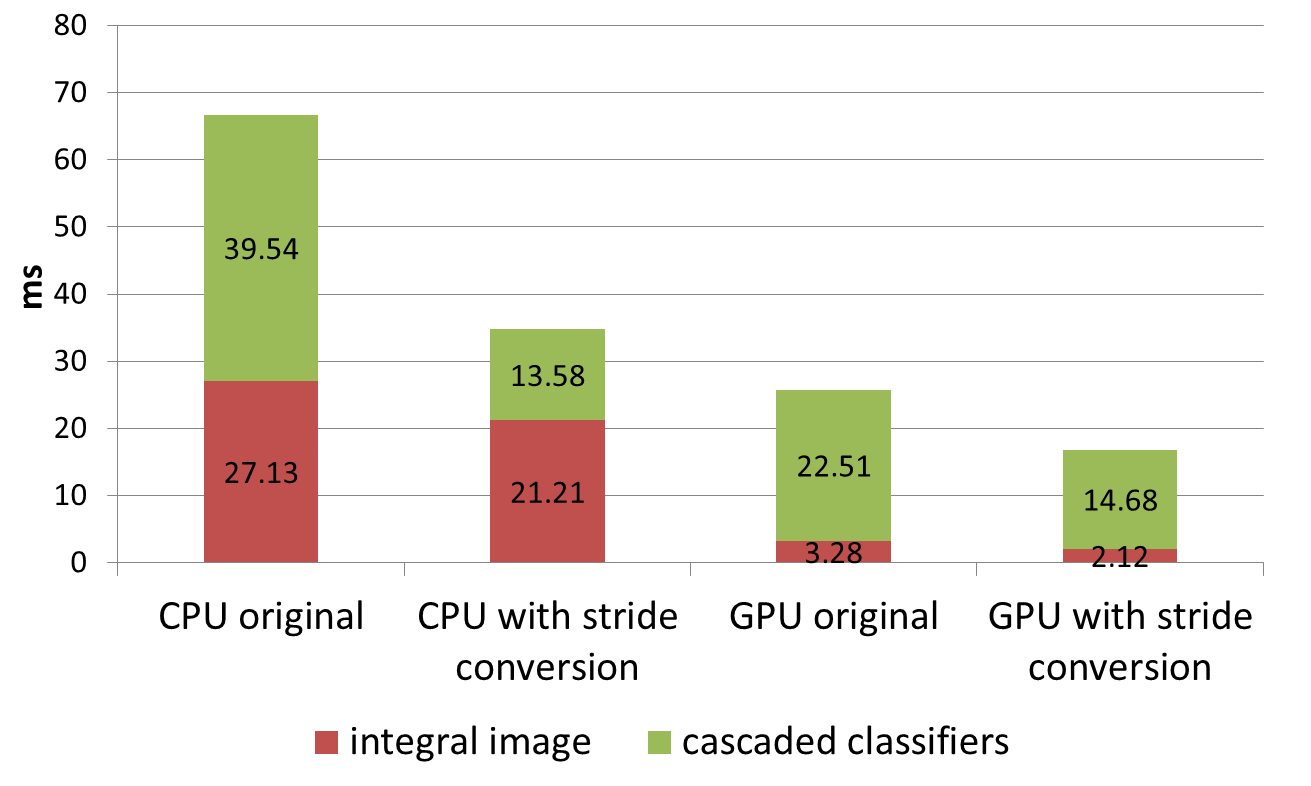
\includegraphics[scale=0.35]{facedetection}
 \caption{Performance comparison of stride converter }
 \label{fig:sparse_total_performance}
 \end{center}
 \end{figure}


\section{Conclusion}
\label{conclusion}
%In a data parallel architecture such as CPU-GPU system, data reorganization is critical.

In this paper,
we proposed a memory access manager which reshapes scalable data layout on-the-fly for each processor in heterogeneous system. Our design support coalescing and sparse storage format conversion. With SC API, programmer can specify non-blocking data transfer and transpose operations in high-level language. Conversion is performed along with data transfer using the proposed ping-pong transpose unit. A control circuit is designed to allow scalable data input.
%In our experiment, our design achieved 68.5 to 2.19 speed up compared to \cite{ASTA} for coalescing issues and \cite{Cusp} for sparse issues.
%Besides, dedicated hardware for conversion provides a significant energy reduction than exploiting general processors.
In our experiment, coalescing conversion achieved 68.5 to 2.19 speed up compared to \cite{ASTA}. Moreover, sparse converter directly transpose COO sparse format to ELL on-the-fly. It improves 339 times than the method which neglecting COO to ELL transformation, and 2.71 times than \cite{Cusp}.





% if have a single appendix:
%\appendix[Proof of the Zonklar Equations]
% or
%\appendix  % for no appendix heading
% do not use \section anymore after \appendix, only \section*
% is possibly needed

% use appendices with more than one appendix
% then use \section to start each appendix
% you must declare a \section before using any
% \subsection or using \label (\appendices by itself
% starts a section numbered zero.)
%


% use section* for acknowledgment
\ifCLASSOPTIONcompsoc
  % The Computer Society usually uses the plural form



% Can use something like this to put references on a page
% by themselves when using endfloat and the captionsoff option.
\ifCLASSOPTIONcaptionsoff
  \newpage
\fi



% trigger a \newpage just before the given reference
% number - used to balance the columns on the last page
% adjust value as needed - may need to be readjusted if
% the document is modified later
%\IEEEtriggeratref{8}
% The "triggered" command can be changed if desired:
%\IEEEtriggercmd{\enlargethispage{-5in}}

% references section

% can use a bibliography generated by BibTeX as a .bbl file
% BibTeX documentation can be easily obtained at:
% http://www.ctan.org/tex-archive/biblio/bibtex/contrib/doc/
% The IEEEtran BibTeX style support page is at:
% http://www.michaelshell.org/tex/ieeetran/bibtex/
\bibliographystyle{IEEEtran}
% argument is your BibTeX string definitions and bibliography database(s)
\bibliography{reference}
%
% <OR> manually copy in the resultant .bbl file
% set second argument of \begin to the number of references
% (used to reserve space for the reference number labels box)

% biography section
%
% If you have an EPS/PDF photo (graphicx package needed) extra braces are
% needed around the contents of the optional argument to biography to prevent
% the LaTeX parser from getting confused when it sees the complicated
% \includegraphics command within an optional argument. (You could create
% your own custom macro containing the \includegraphics command to make things
% simpler here.)
%\begin{IEEEbiography}[{\includegraphics[width=1in,height=1.25in,clip,keepaspectratio]{mshell}}]{Michael Shell}
% or if you just want to reserve a space for a photo:

%\begin{IEEEbiography}{Michael Shell}
%Biography text here.
%\end{IEEEbiography}

% if you will not have a photo at all:
%\begin{IEEEbiographynophoto}{John Doe}
%Biography text here.
%\end{IEEEbiographynophoto}

% insert where needed to balance the two columns on the last page with
% biographies
%\newpage

%\begin{IEEEbiographynophoto}{Jane Doe}
%Biography text here.
%\end{IEEEbiographynophoto}

% You can push biographies down or up by placing
% a \vfill before or after them. The appropriate
% use of \vfill depends on what kind of text is
% on the last page and whether or not the columns
% are being equalized.

%\vfill

% Can be used to pull up biographies so that the bottom of the last one
% is flush with the other column.
%\enlargethispage{-5in}



% that's all folks
\end{document}


